\chapter{Problématique : Images des plateformes}
\label{annexe:problematique}

\section{Practice-it}

\begin{figure}[H]
    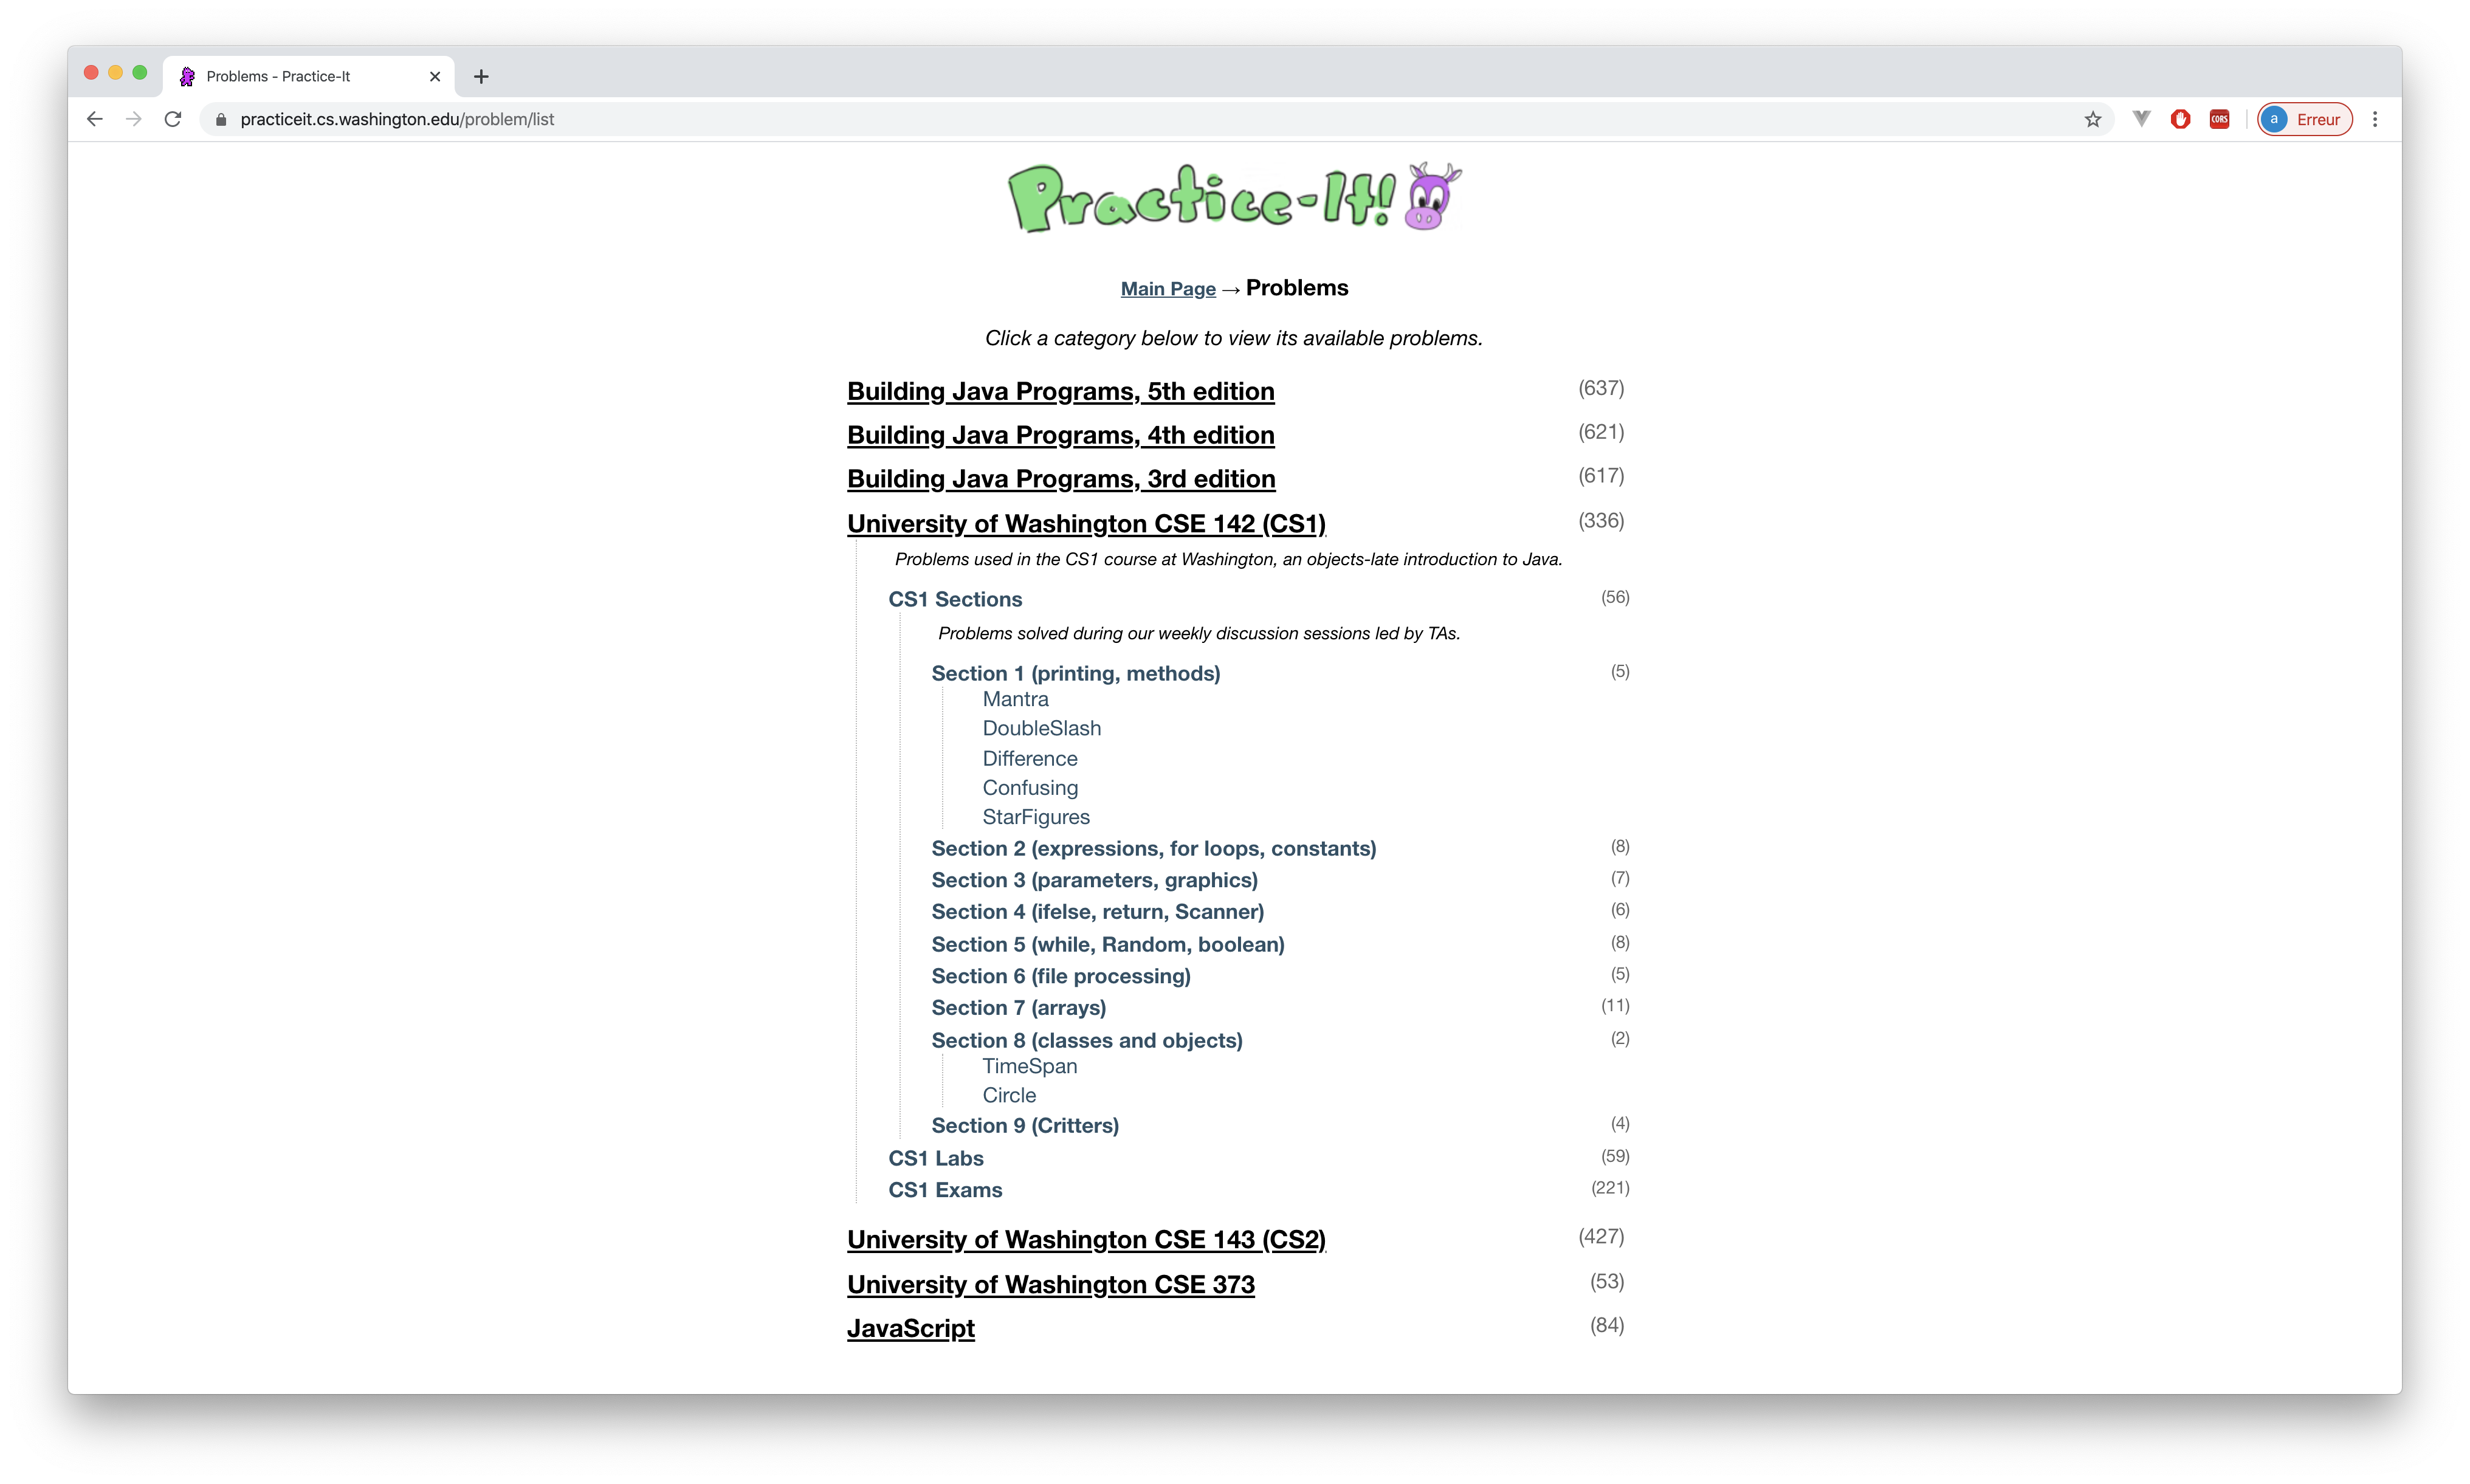
\includegraphics[width=\textwidth,height=0.6\textheight,keepaspectratio]{images/comparison/practice-it-1.png}
    \centering
    \caption[Practice-it : page principale pour rechercher un problème]{Page principale pour rechercher un problème}
\end{figure}

\begin{figure}[H]
    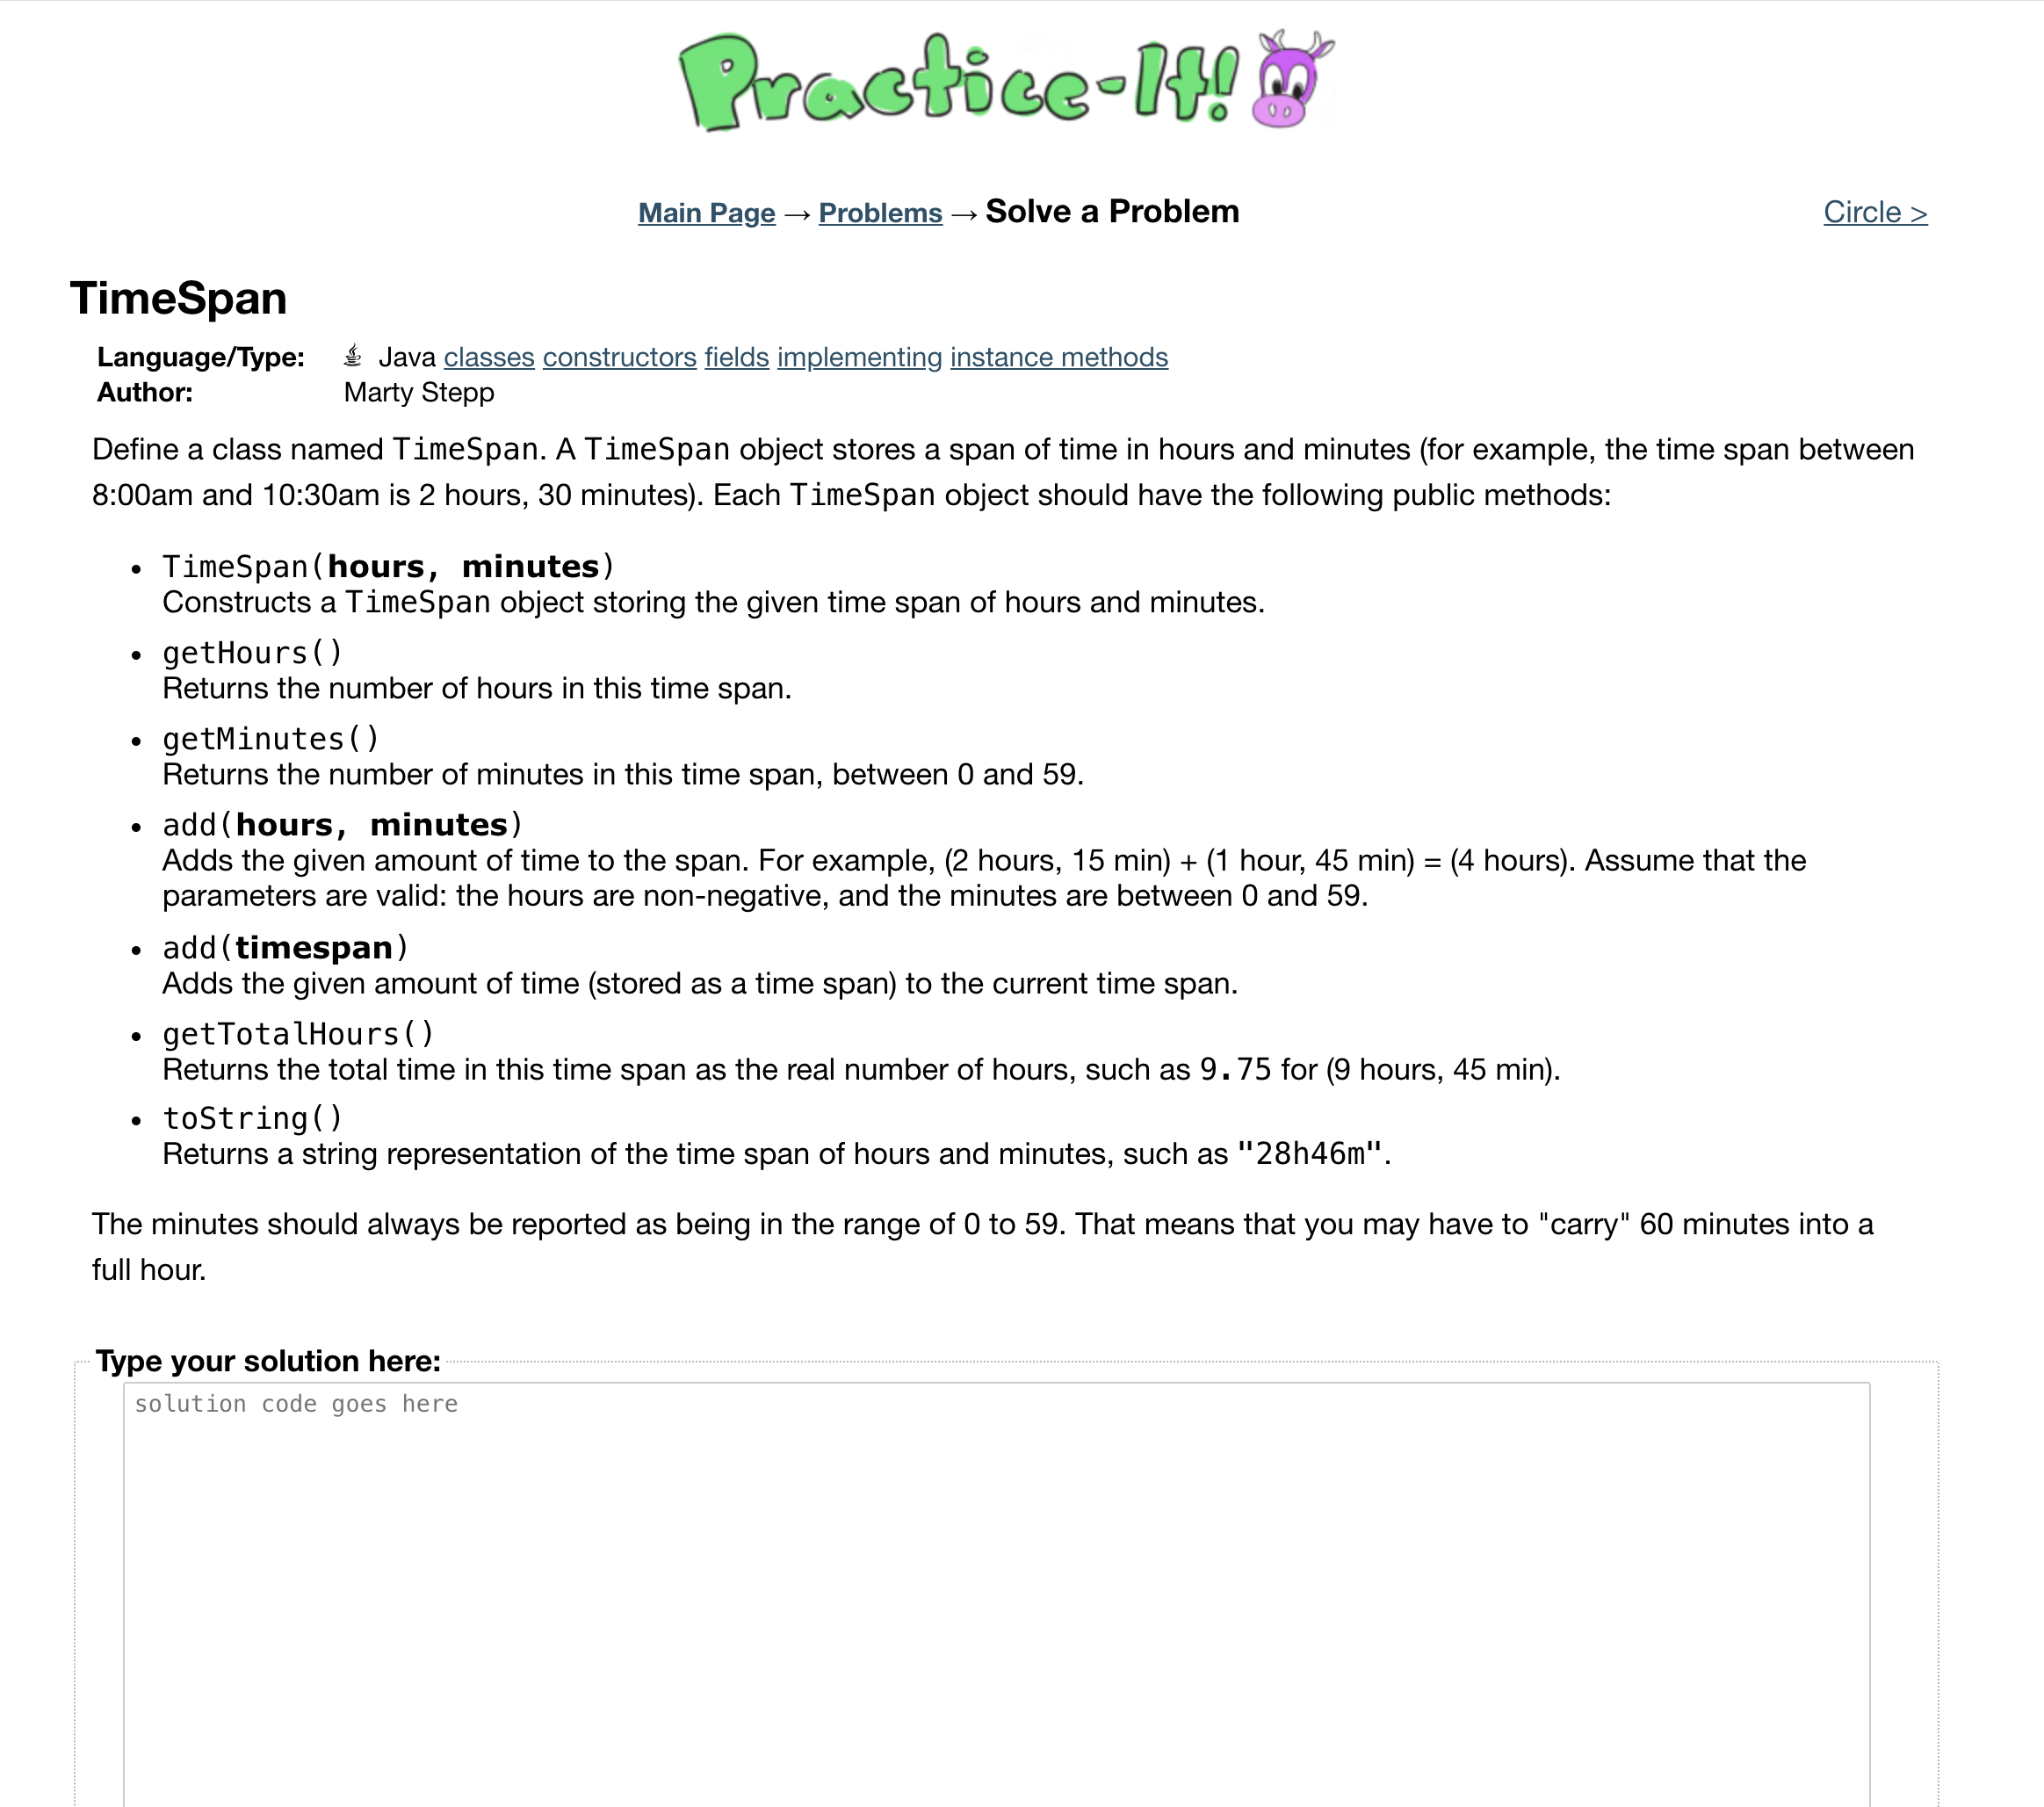
\includegraphics[width=\textwidth,height=0.6\textheight,keepaspectratio]{images/comparison/practice-it-2.png}
    \centering
    \caption[Practice-it : page d'un problème]{Page d'un problème}
\end{figure}

\begin{figure}[H]
    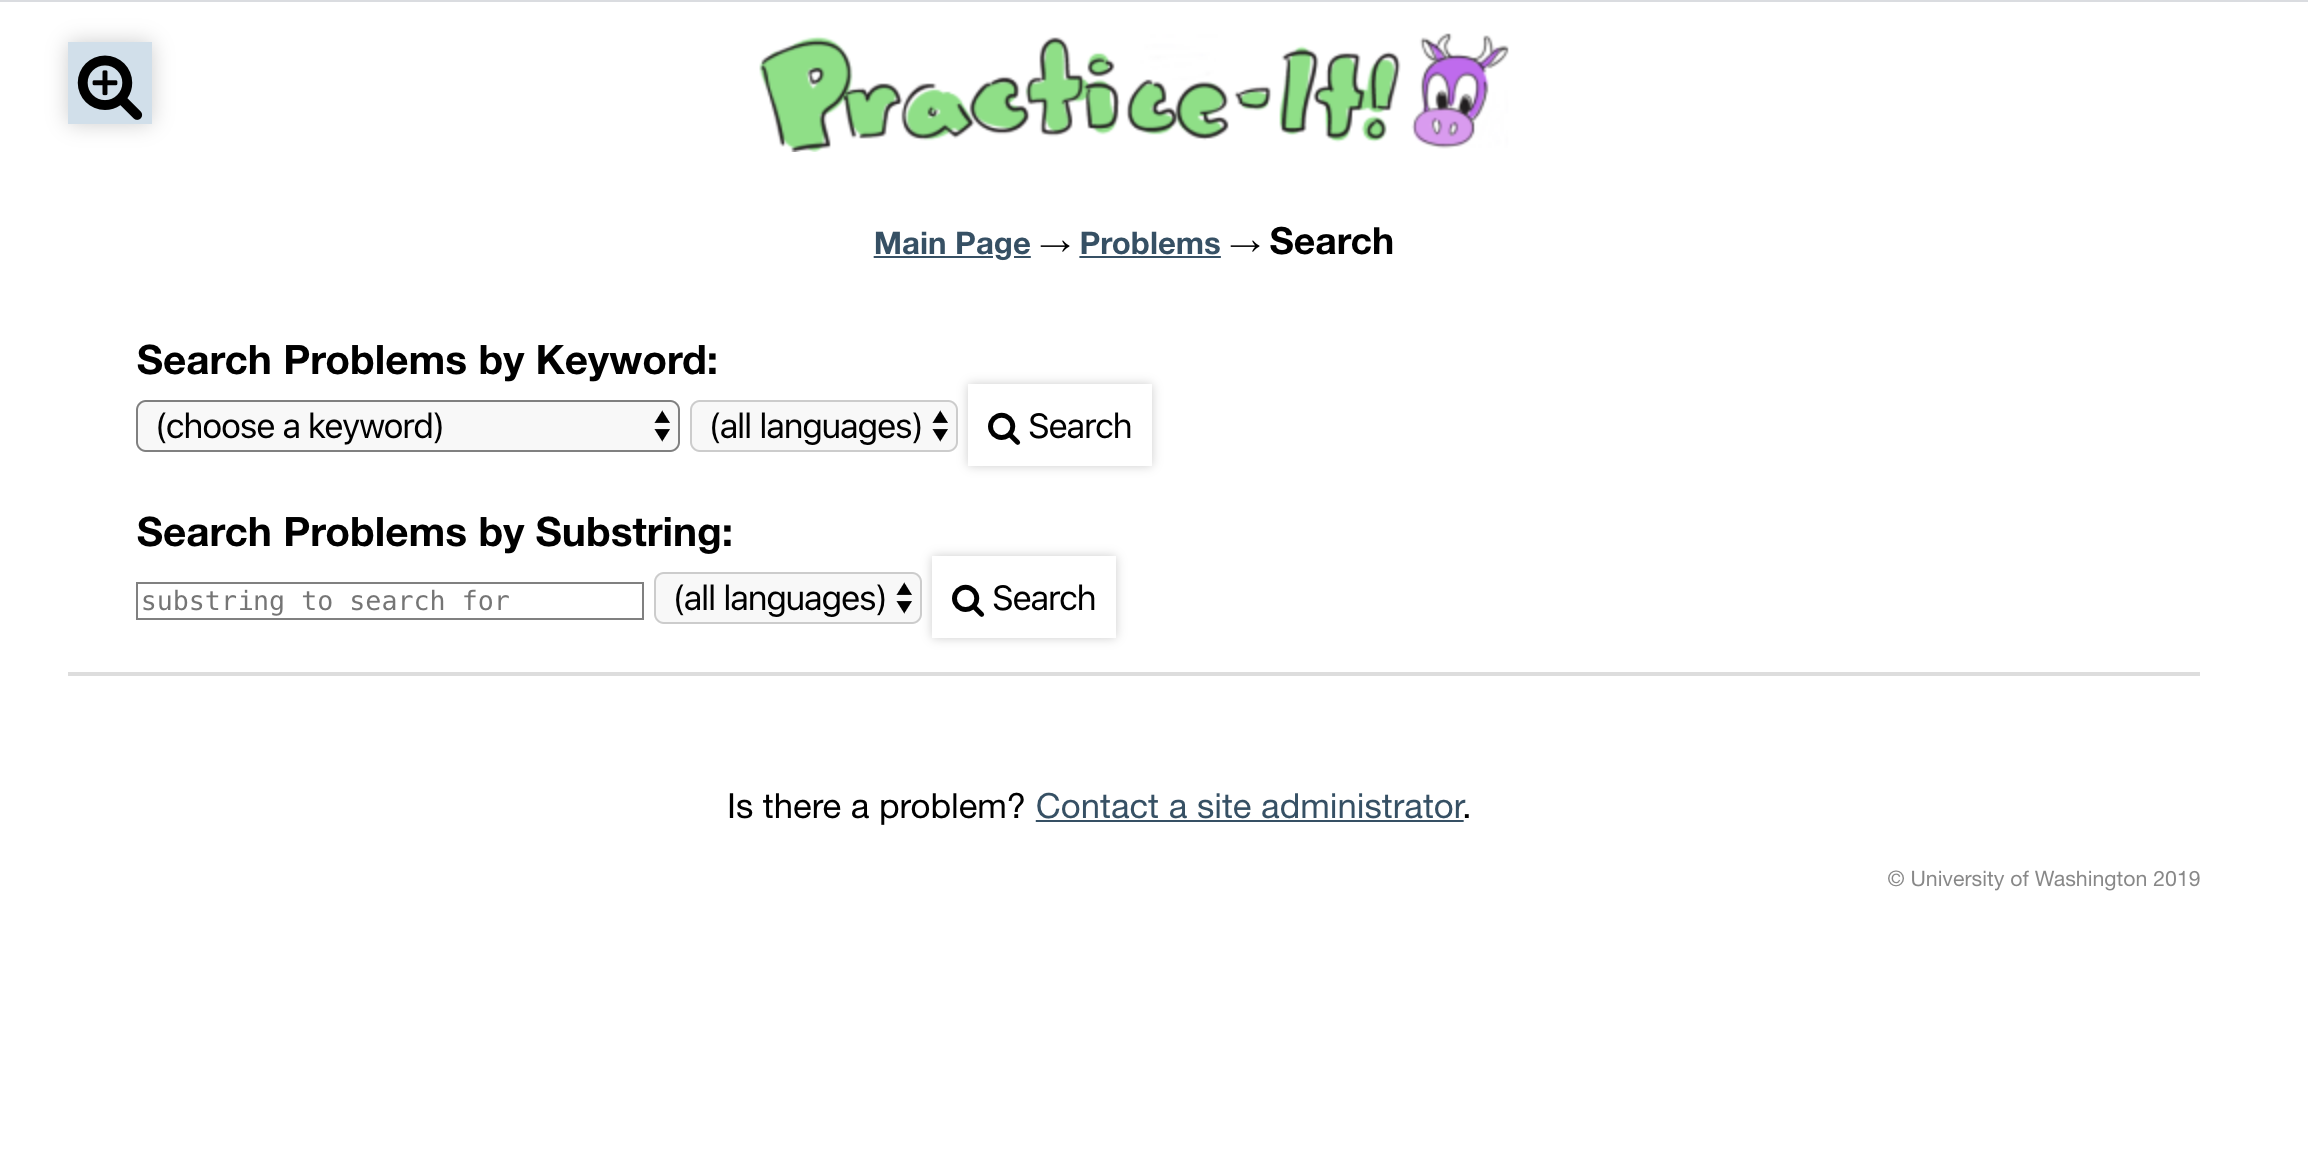
\includegraphics[width=\textwidth,height=0.35\textheight,keepaspectratio]{images/comparison/practice-it-3.png}
    \centering
    \caption[Practice-it : recherche avancée]{Recherche avancée}
\end{figure}

\section{Hackerrank}

\begin{figure}[H]
    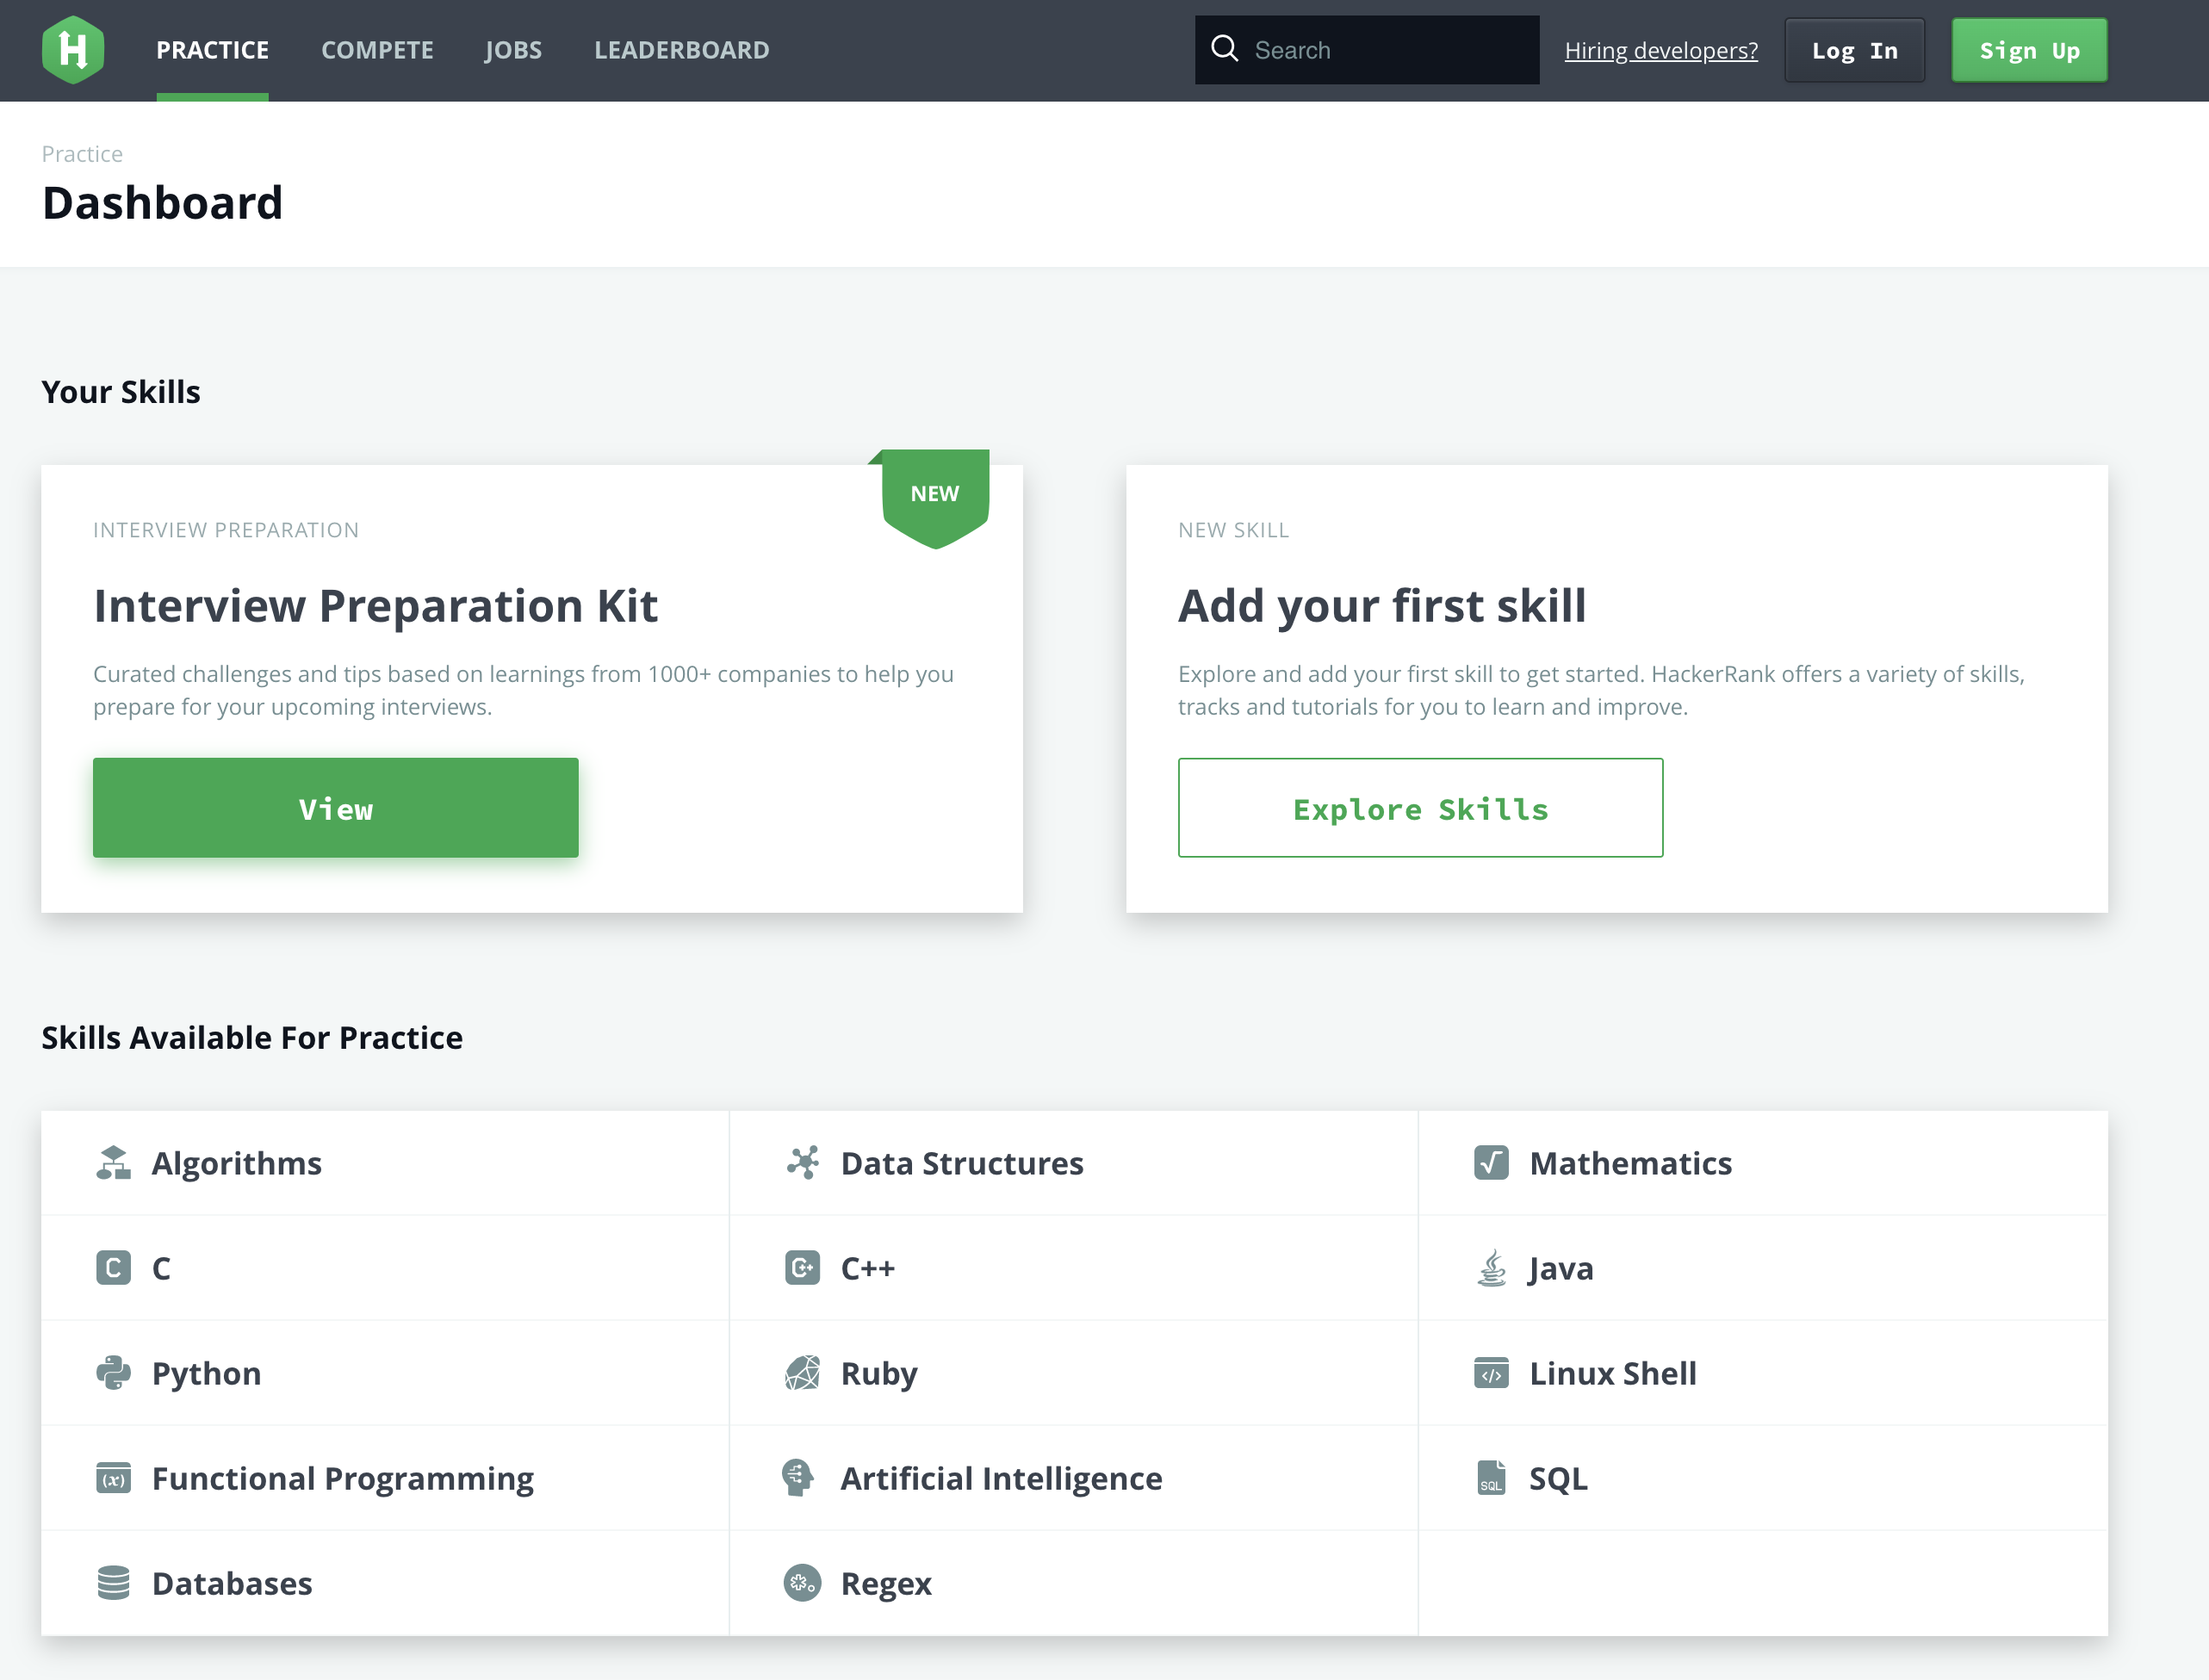
\includegraphics[width=\textwidth,height=0.35\textheight,keepaspectratio]{images/comparison/hacker-1.png}
    \centering
    \caption[Hackerrank : tableau de bord]{Tableau de bord}
\end{figure}

\begin{figure}[H]
    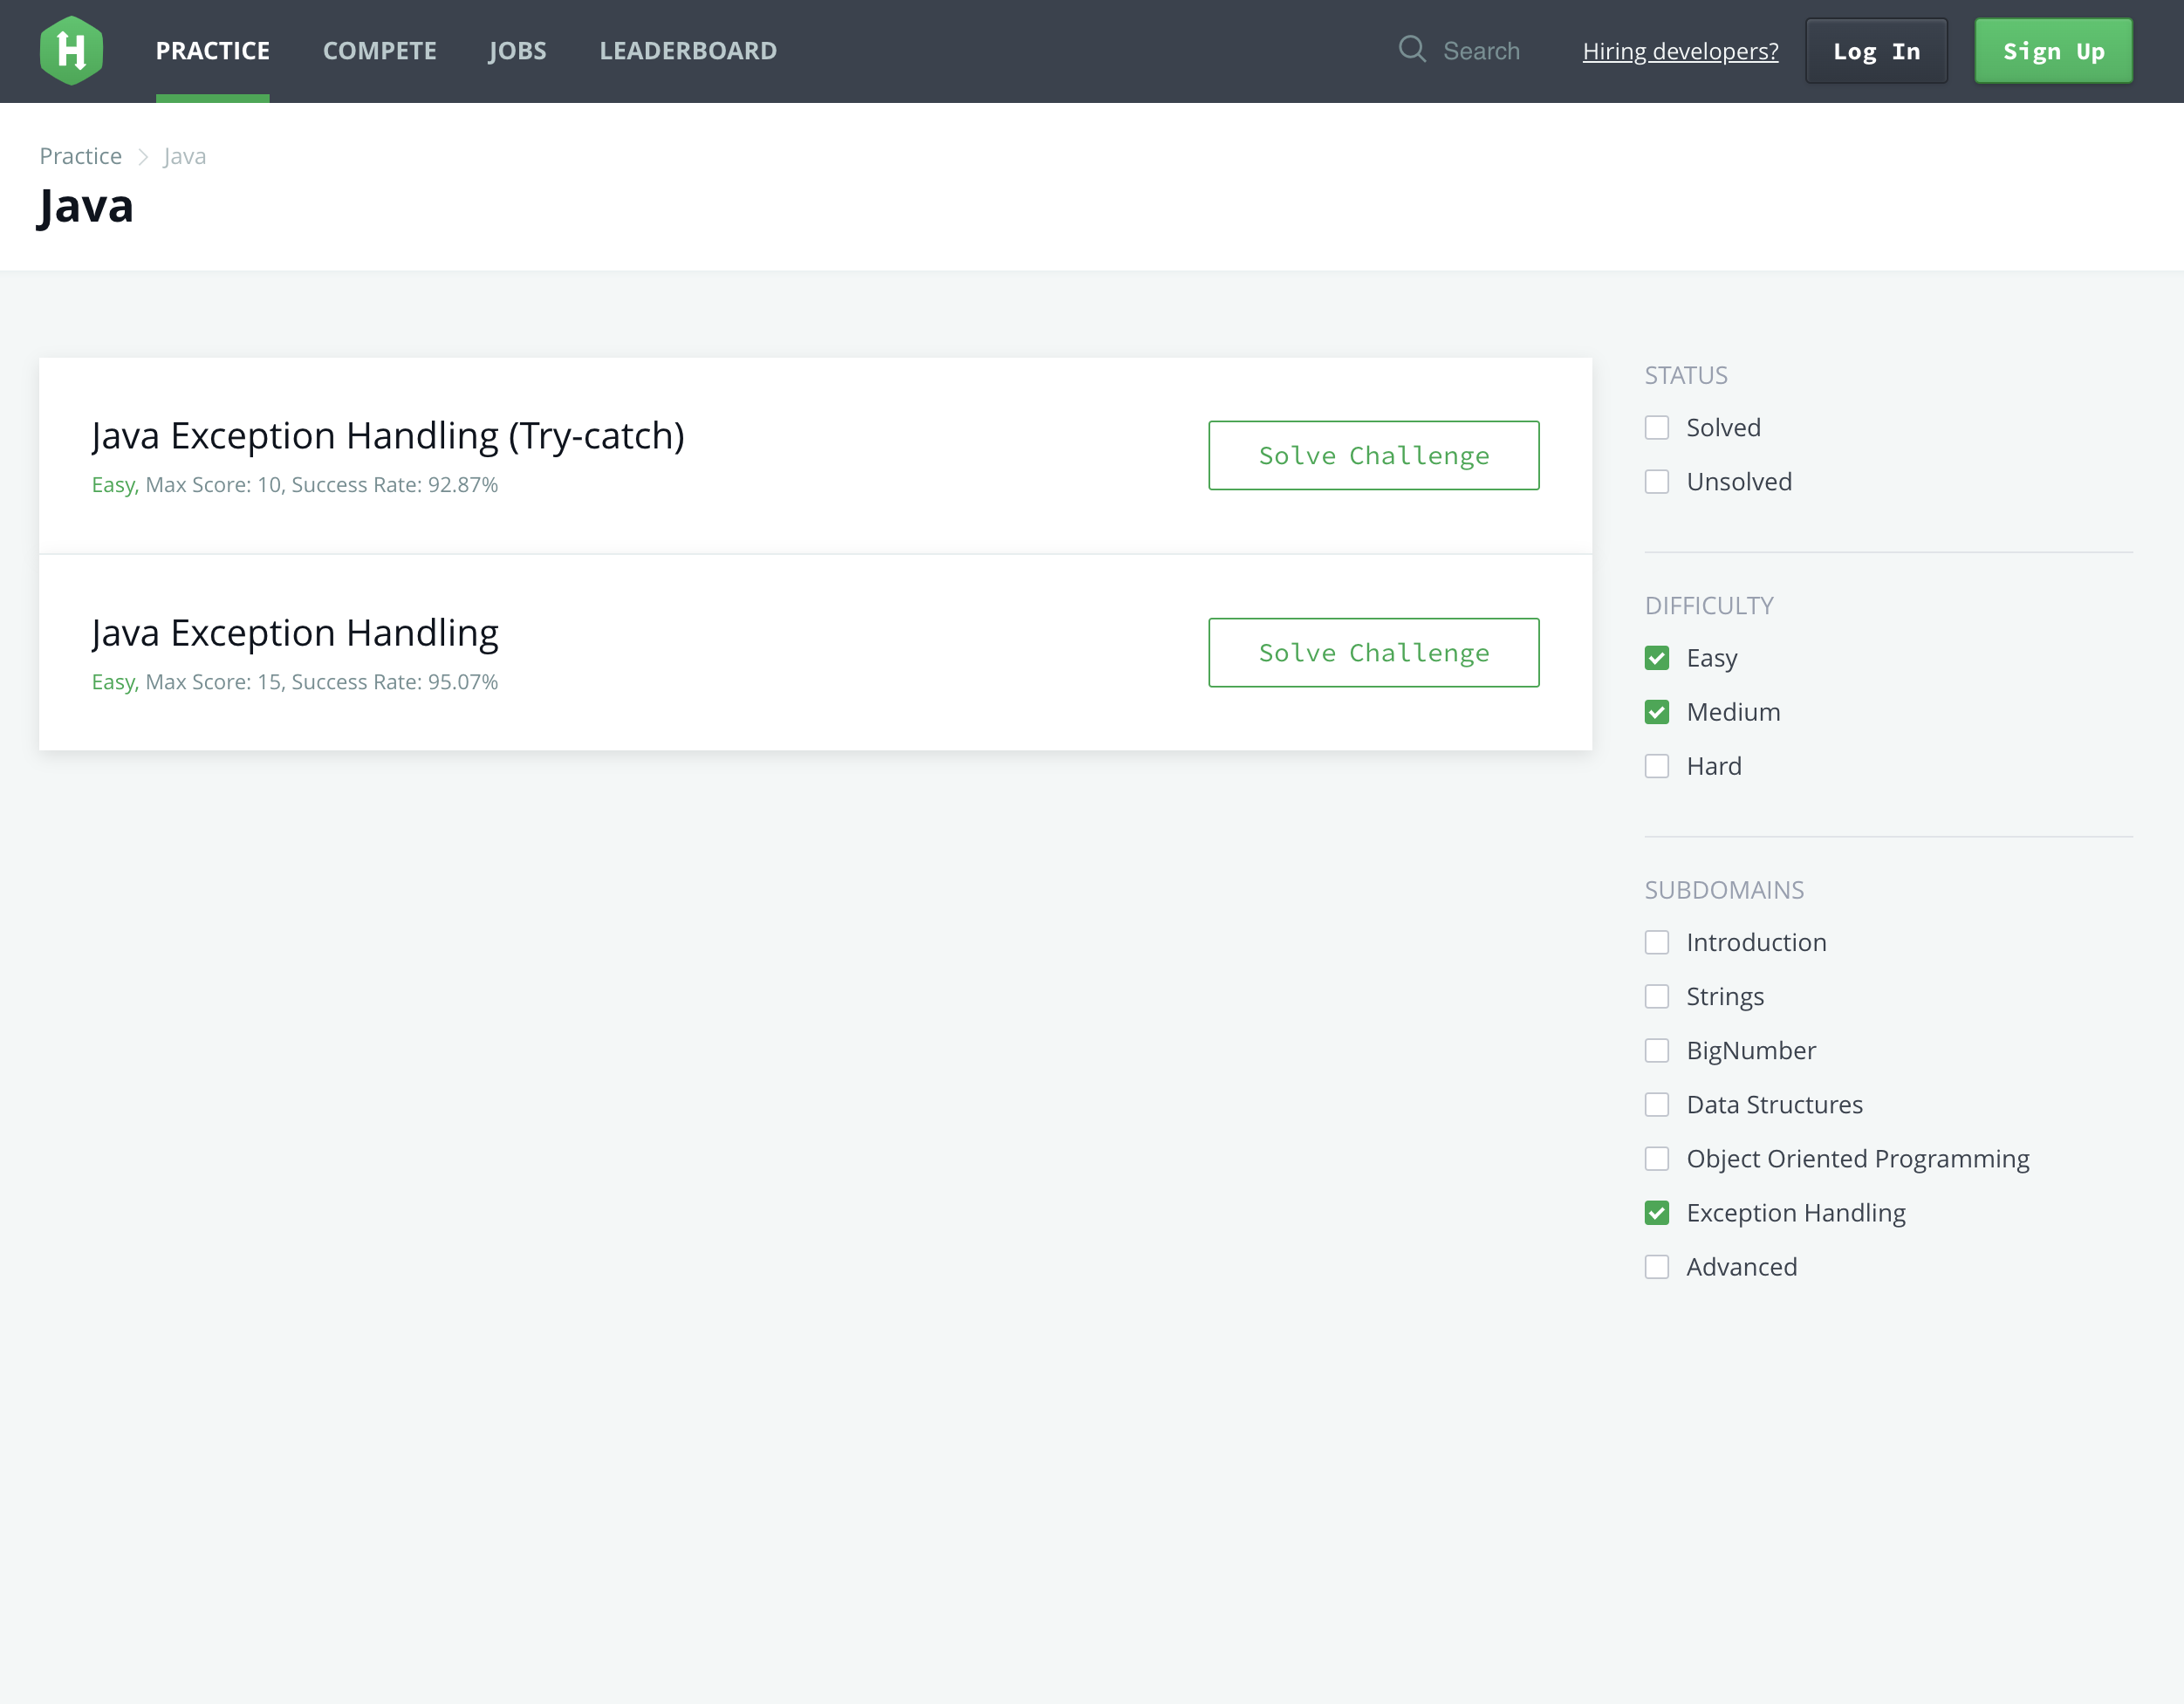
\includegraphics[width=\textwidth,height=0.35\textheight,keepaspectratio]{images/comparison/hacker-2.png}
    \centering
    \caption[Hackerrank : page pour rechercher un problème]{Page pour rechercher un problème}
\end{figure}

\begin{figure}[H]
    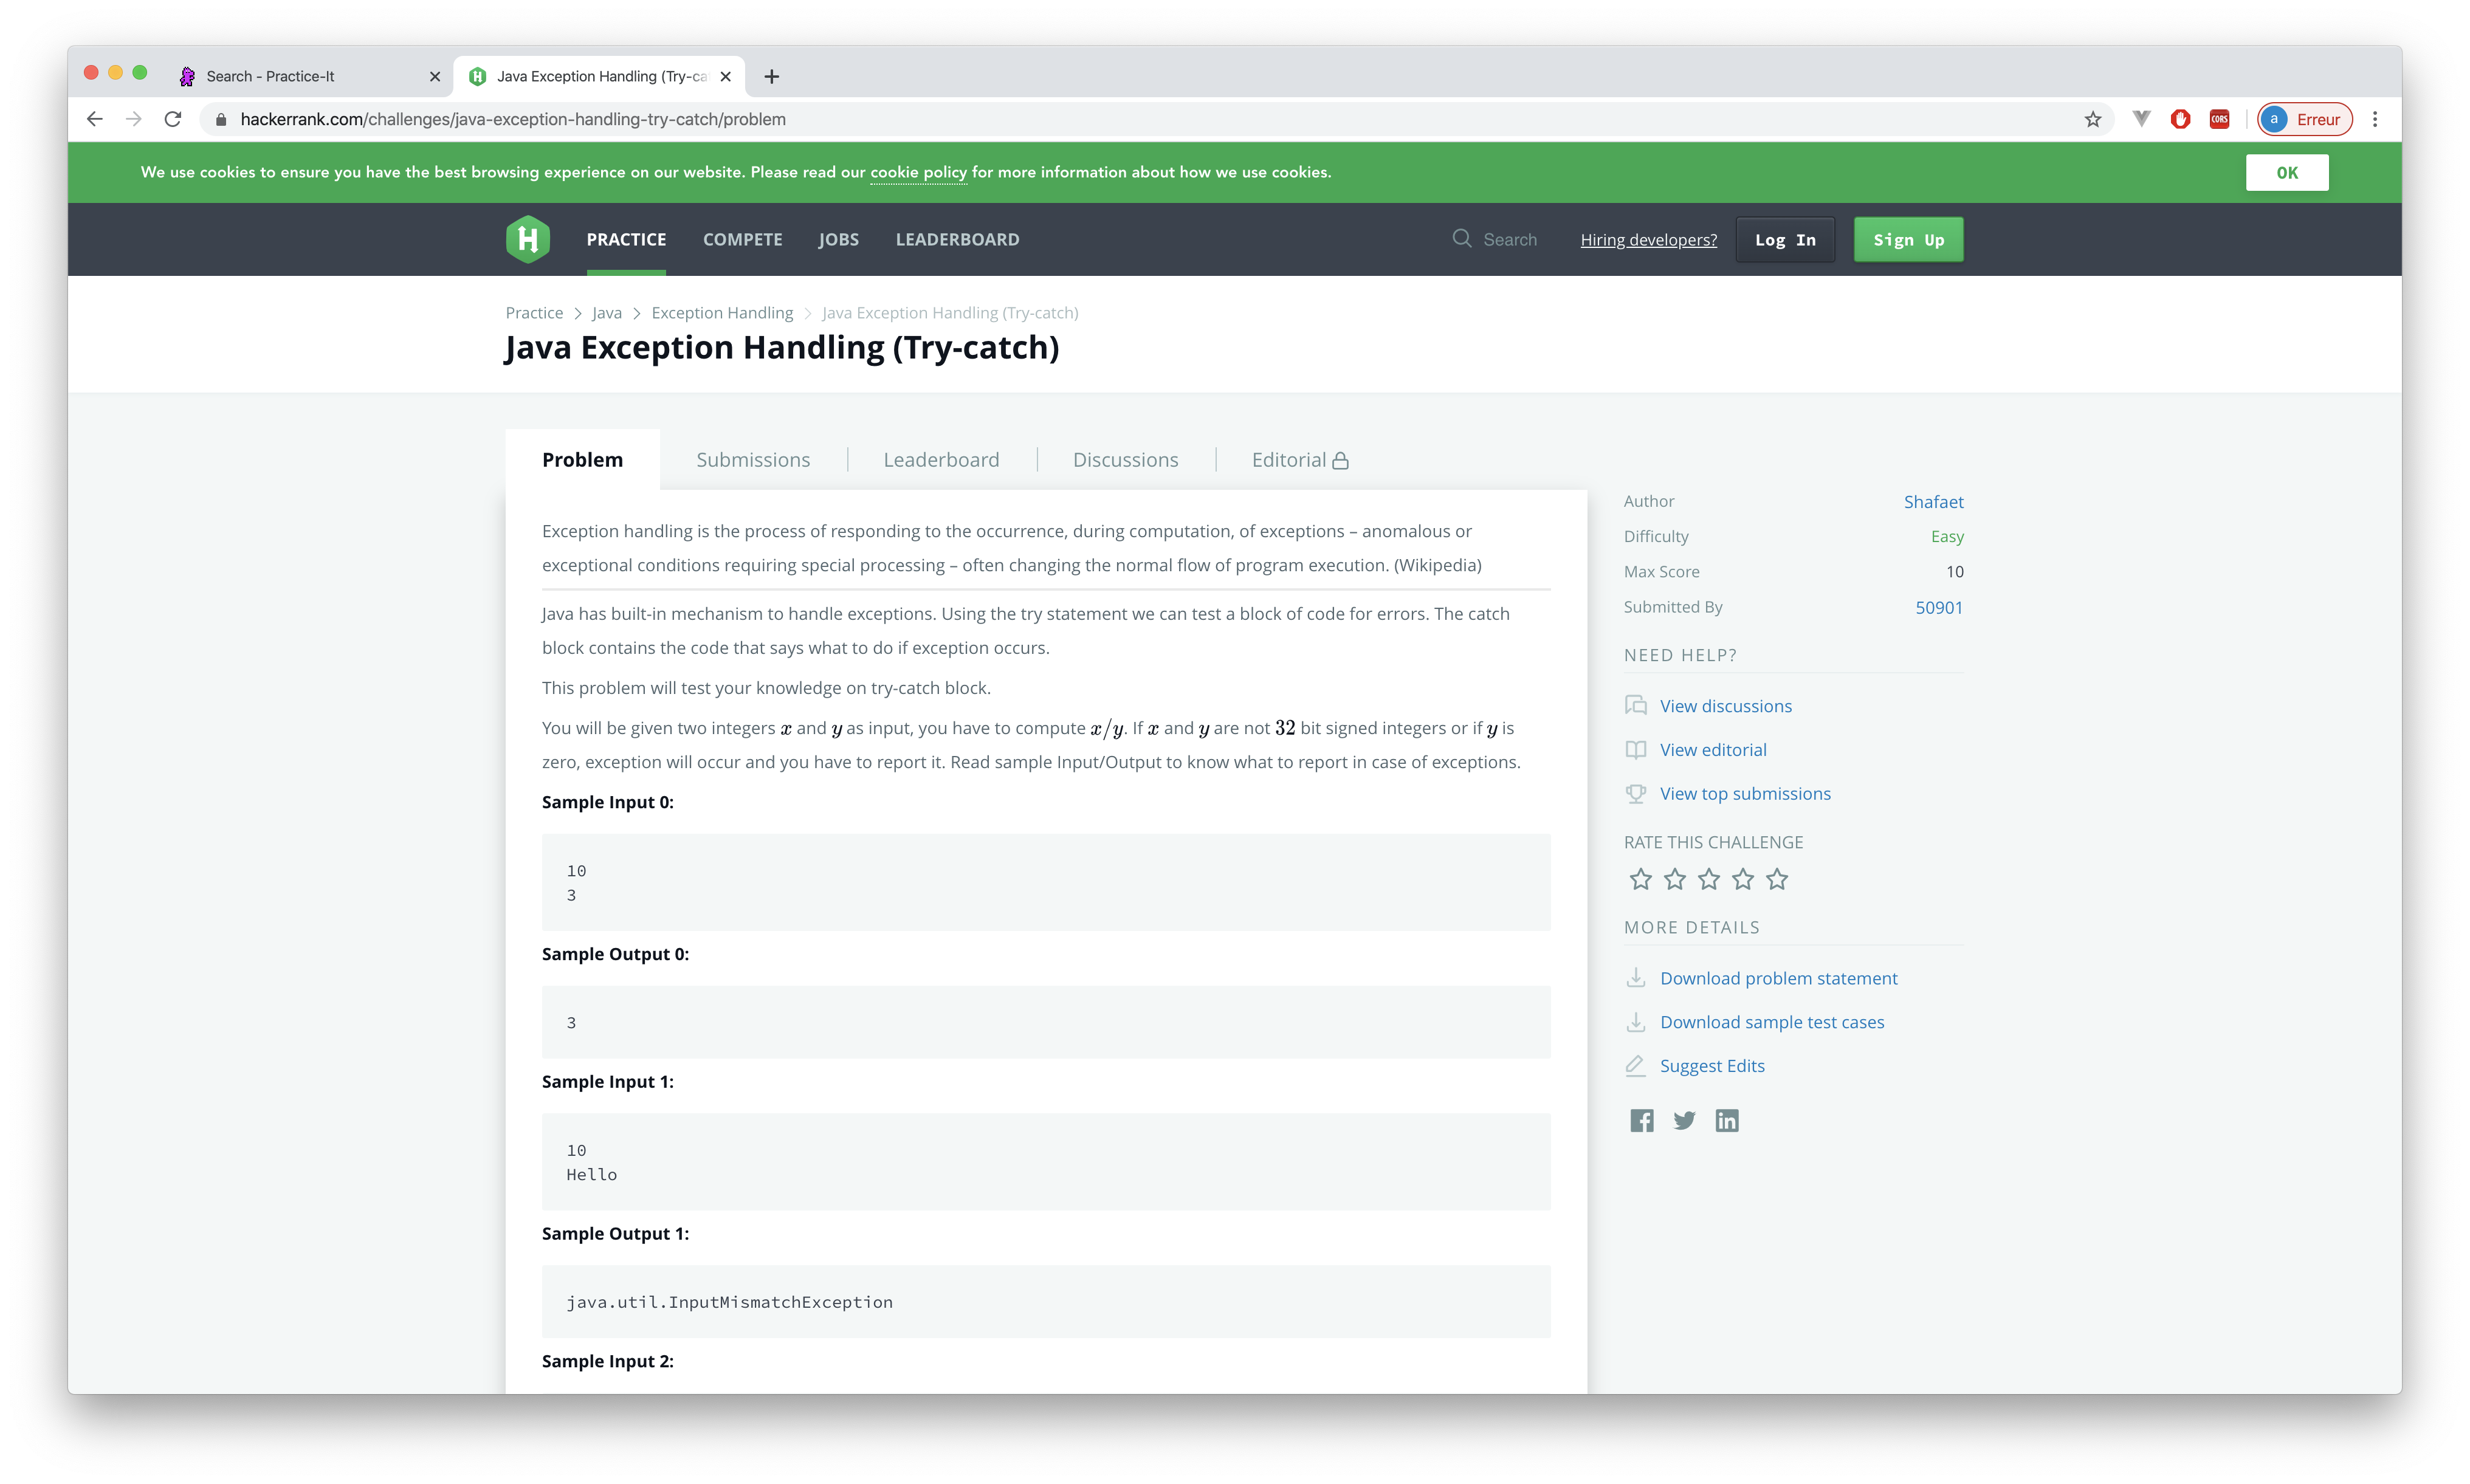
\includegraphics[width=\textwidth,height=0.35\textheight,keepaspectratio]{images/comparison/hacker-3.png}
    \centering
    \caption[Hackerrank : page d'un challenge]{Page d'un challenge}
\end{figure}

\section{Leetcode}

\begin{figure}[H]
    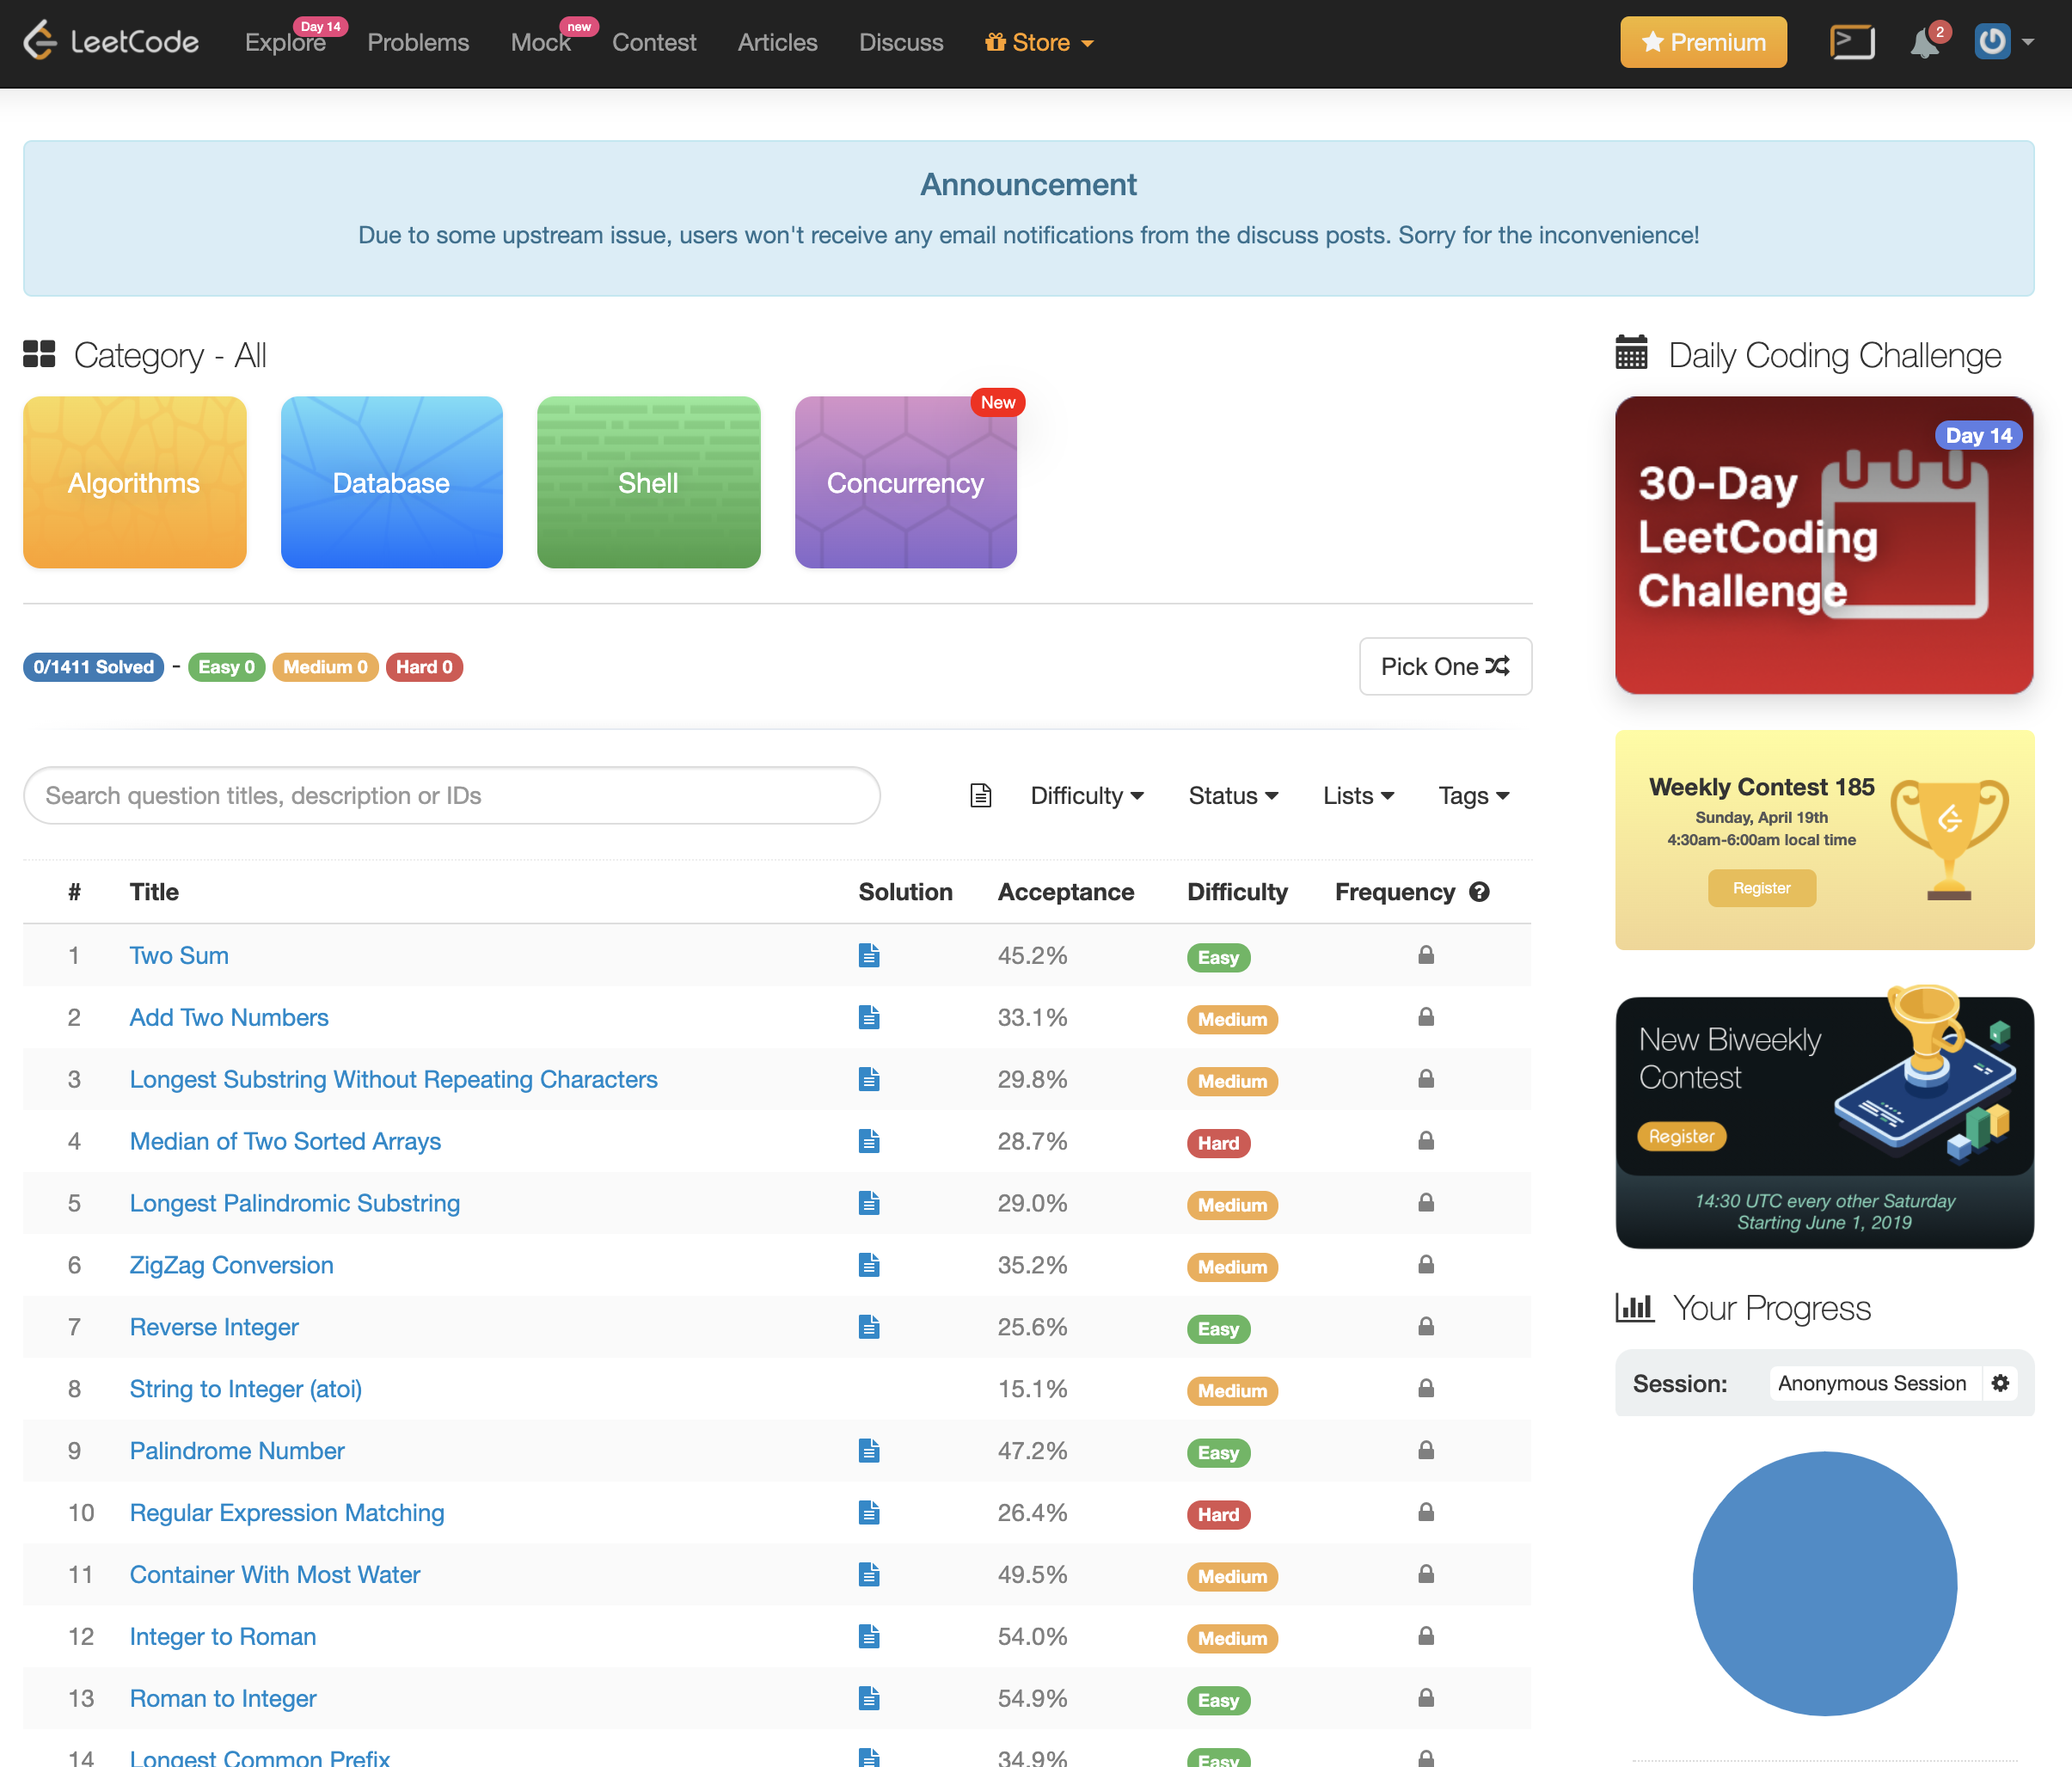
\includegraphics[width=\textwidth,height=0.6\textheight,keepaspectratio]{images/comparison/leetcode-1.png}
    \centering
    \caption[Leetcode : page de recherche de problèmes]{Page de recherche de problèmes}
\end{figure}

\begin{figure}[H]
    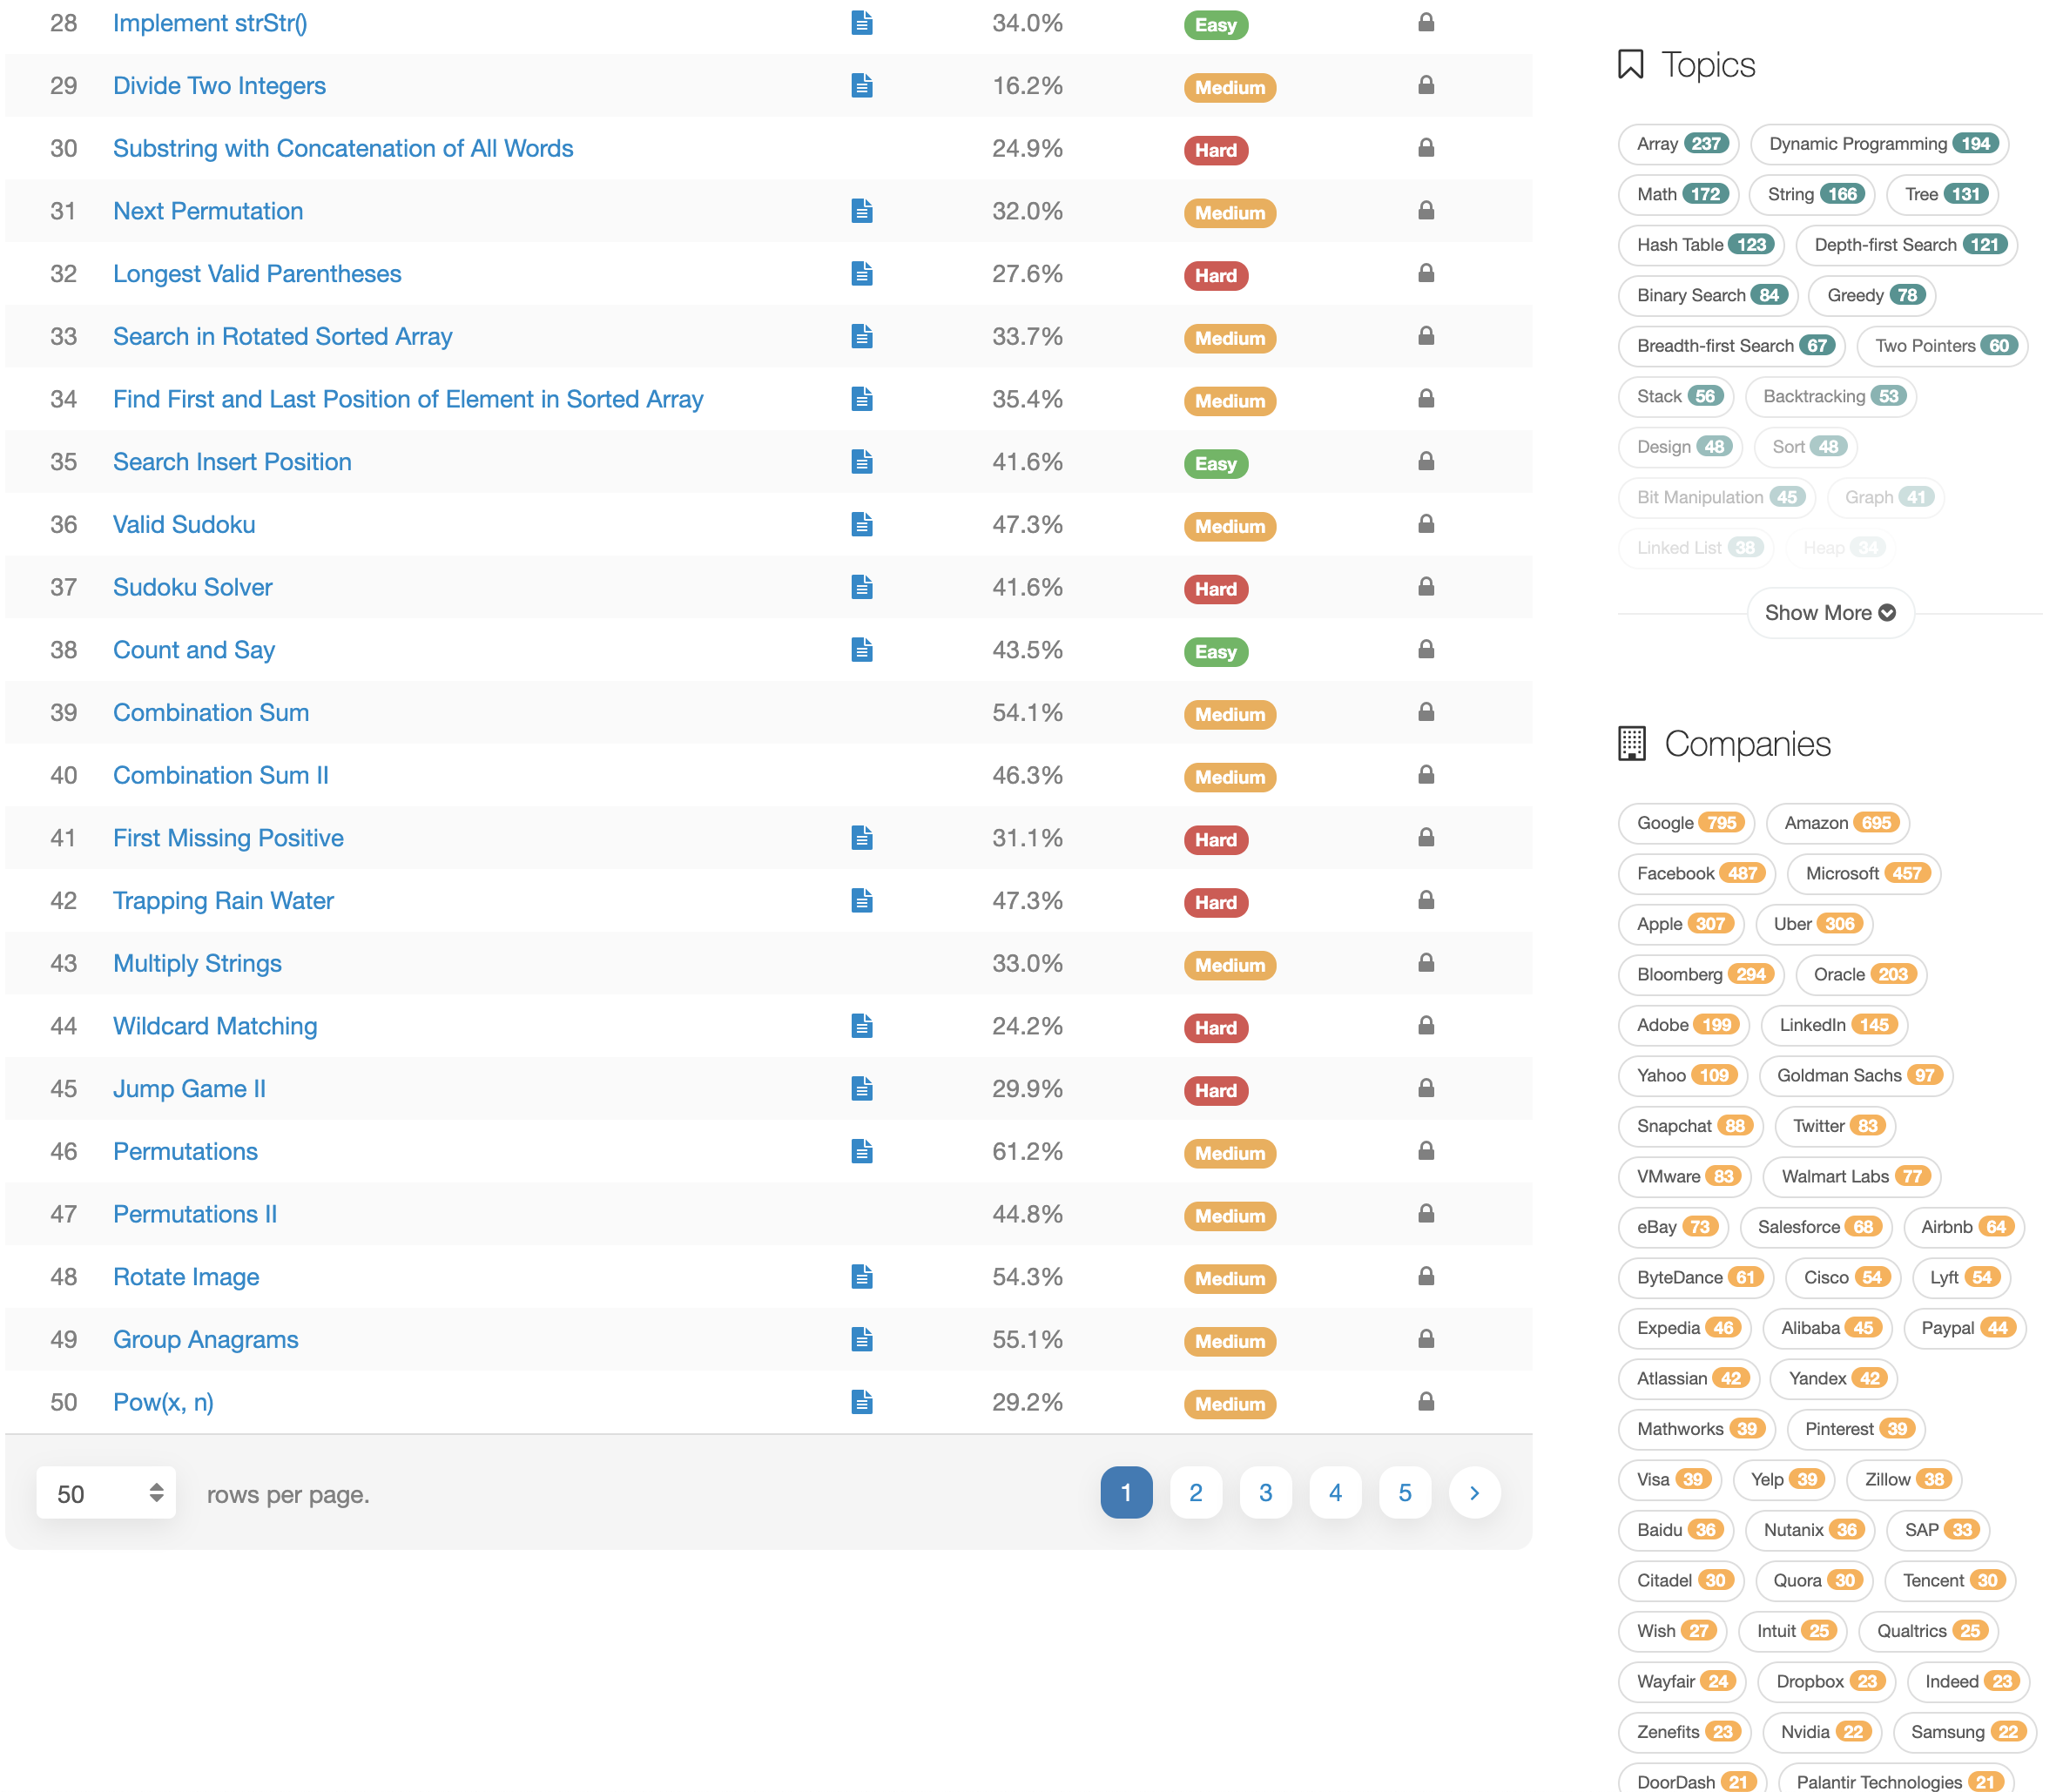
\includegraphics[width=\textwidth,height=0.6\textheight,keepaspectratio]{images/comparison/leetcode-2.png}
    \centering
    \caption[Leetcode : quelques \glspl{tag} disponibles sur le côté droit]{Quelques \glspl{tag} disponibles sur le côté droit}
\end{figure}

\begin{figure}[H]
    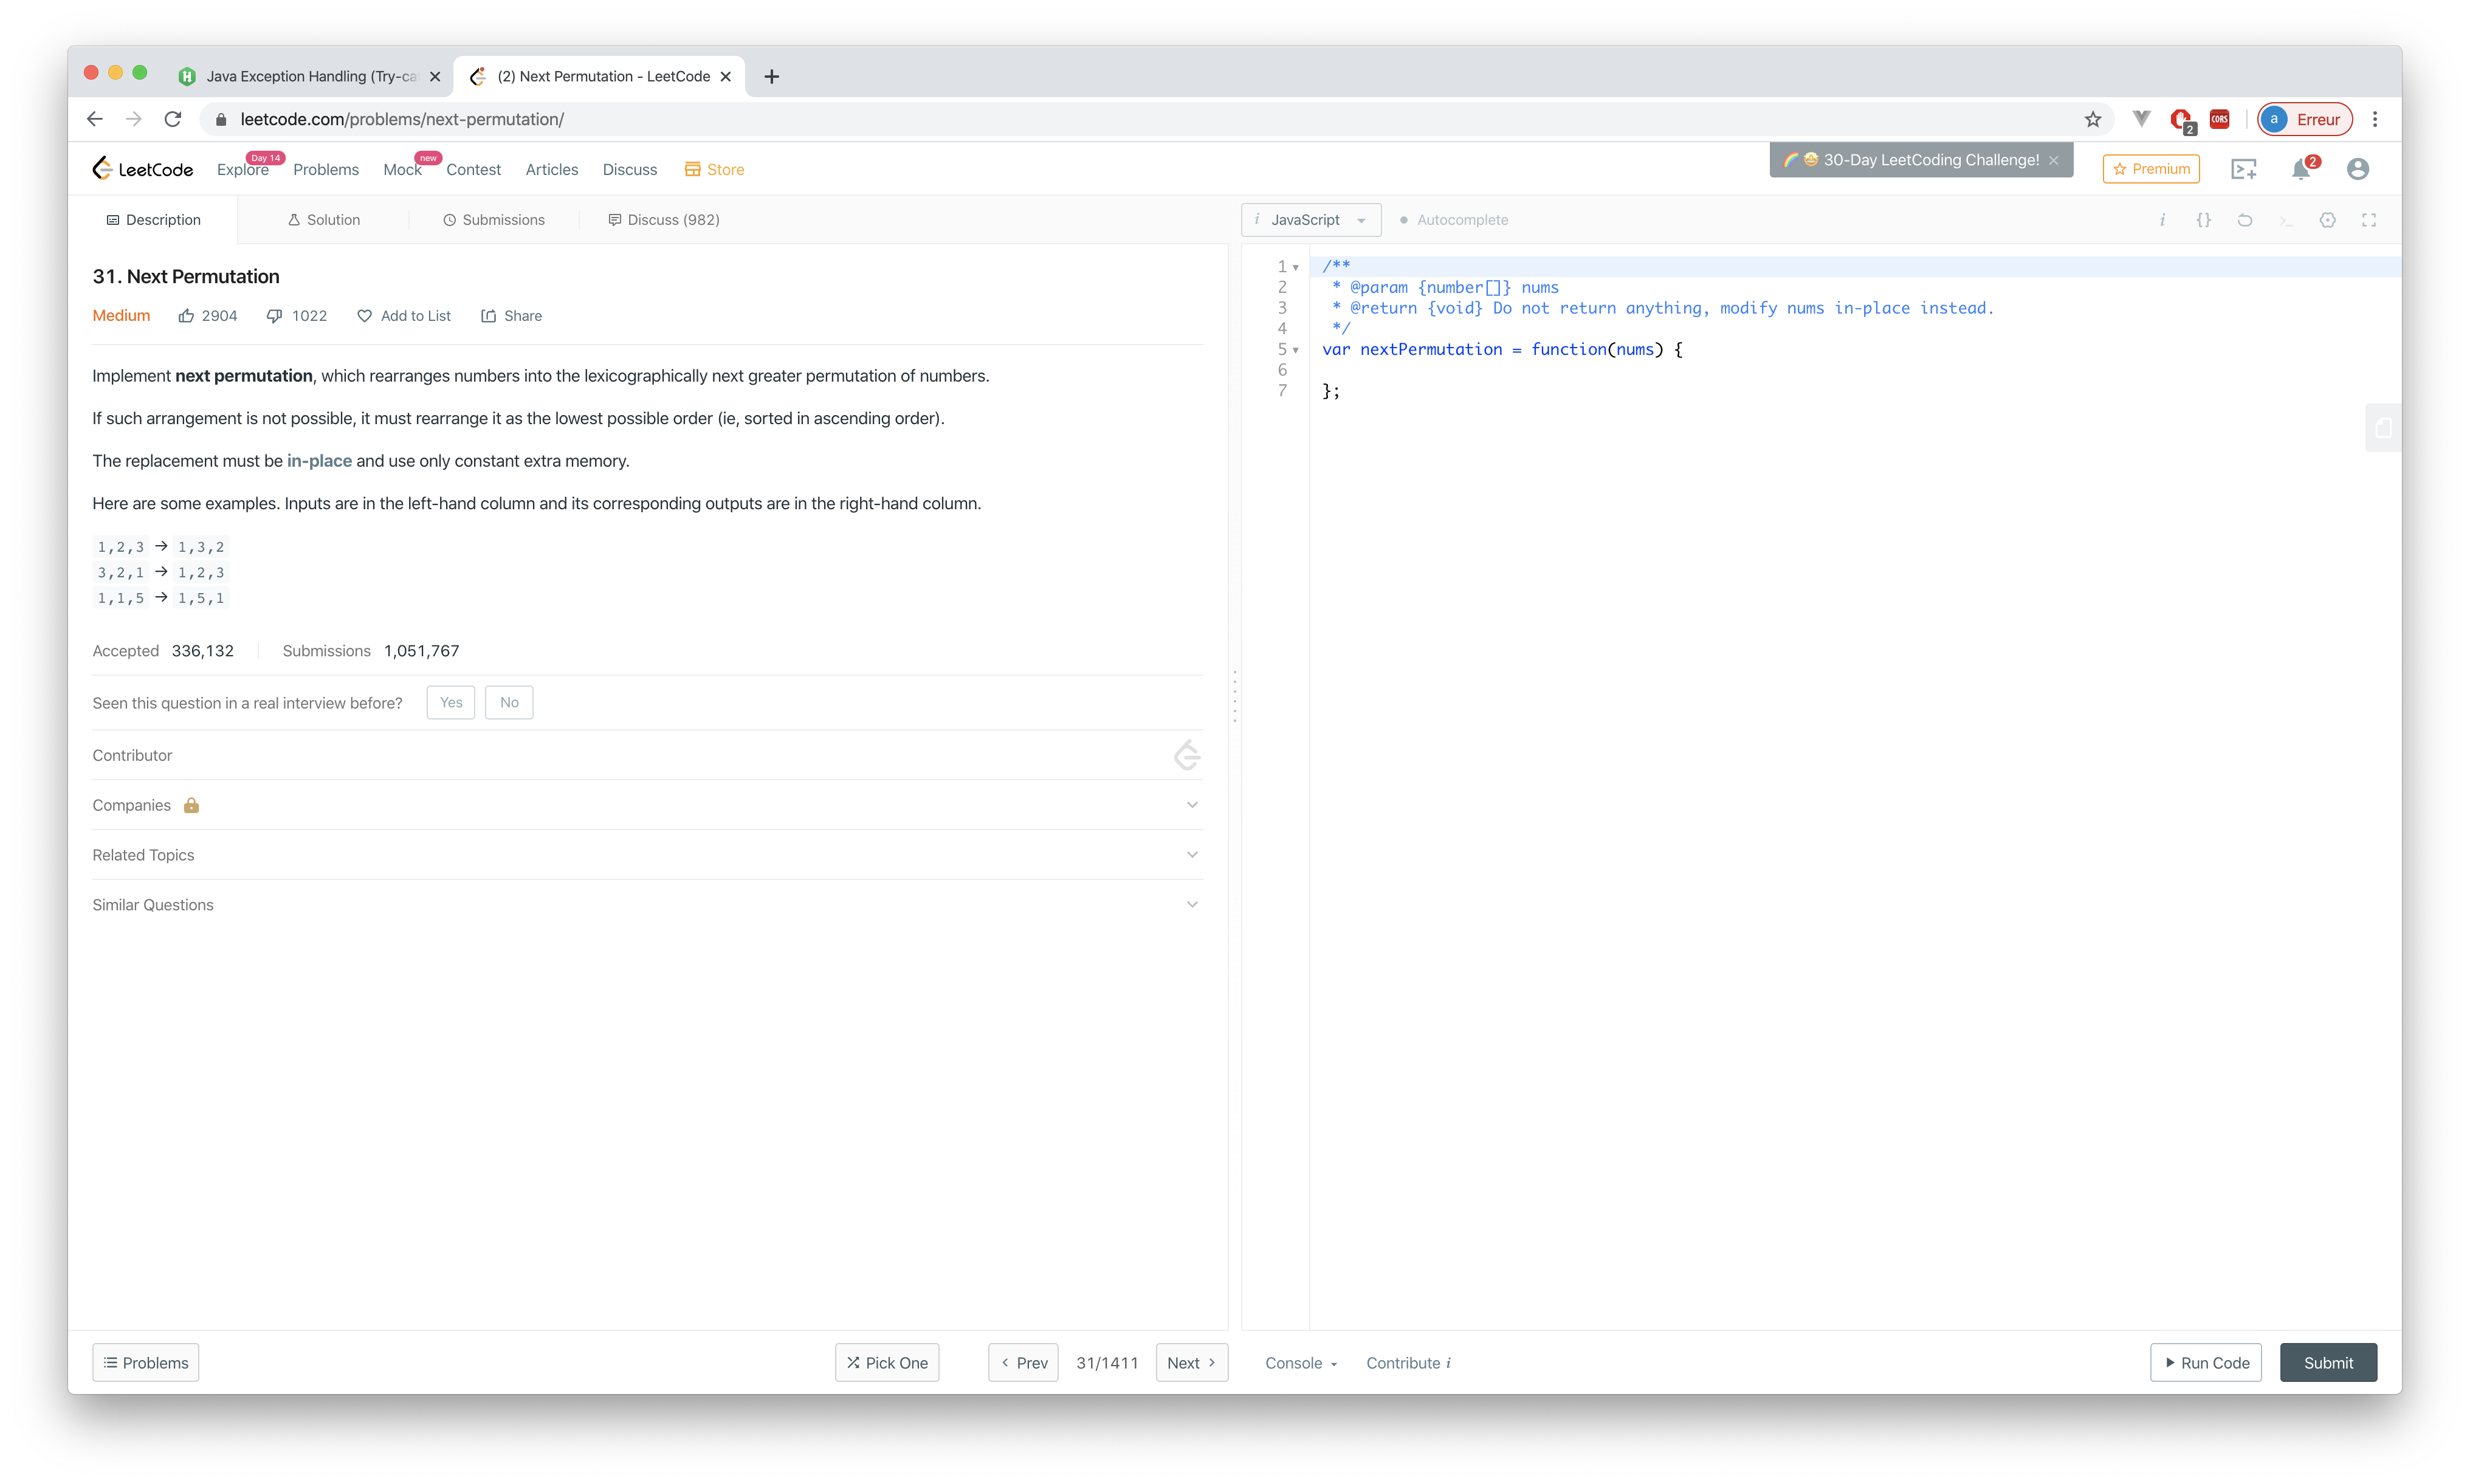
\includegraphics[width=\textwidth,height=0.35\textheight,keepaspectratio]{images/comparison/leetcode-3.png}
    \centering
    \caption[Leetcode : page d'un problème]{Page d'un problème}
\end{figure}


\section{Codeforces}

\begin{figure}[H]
    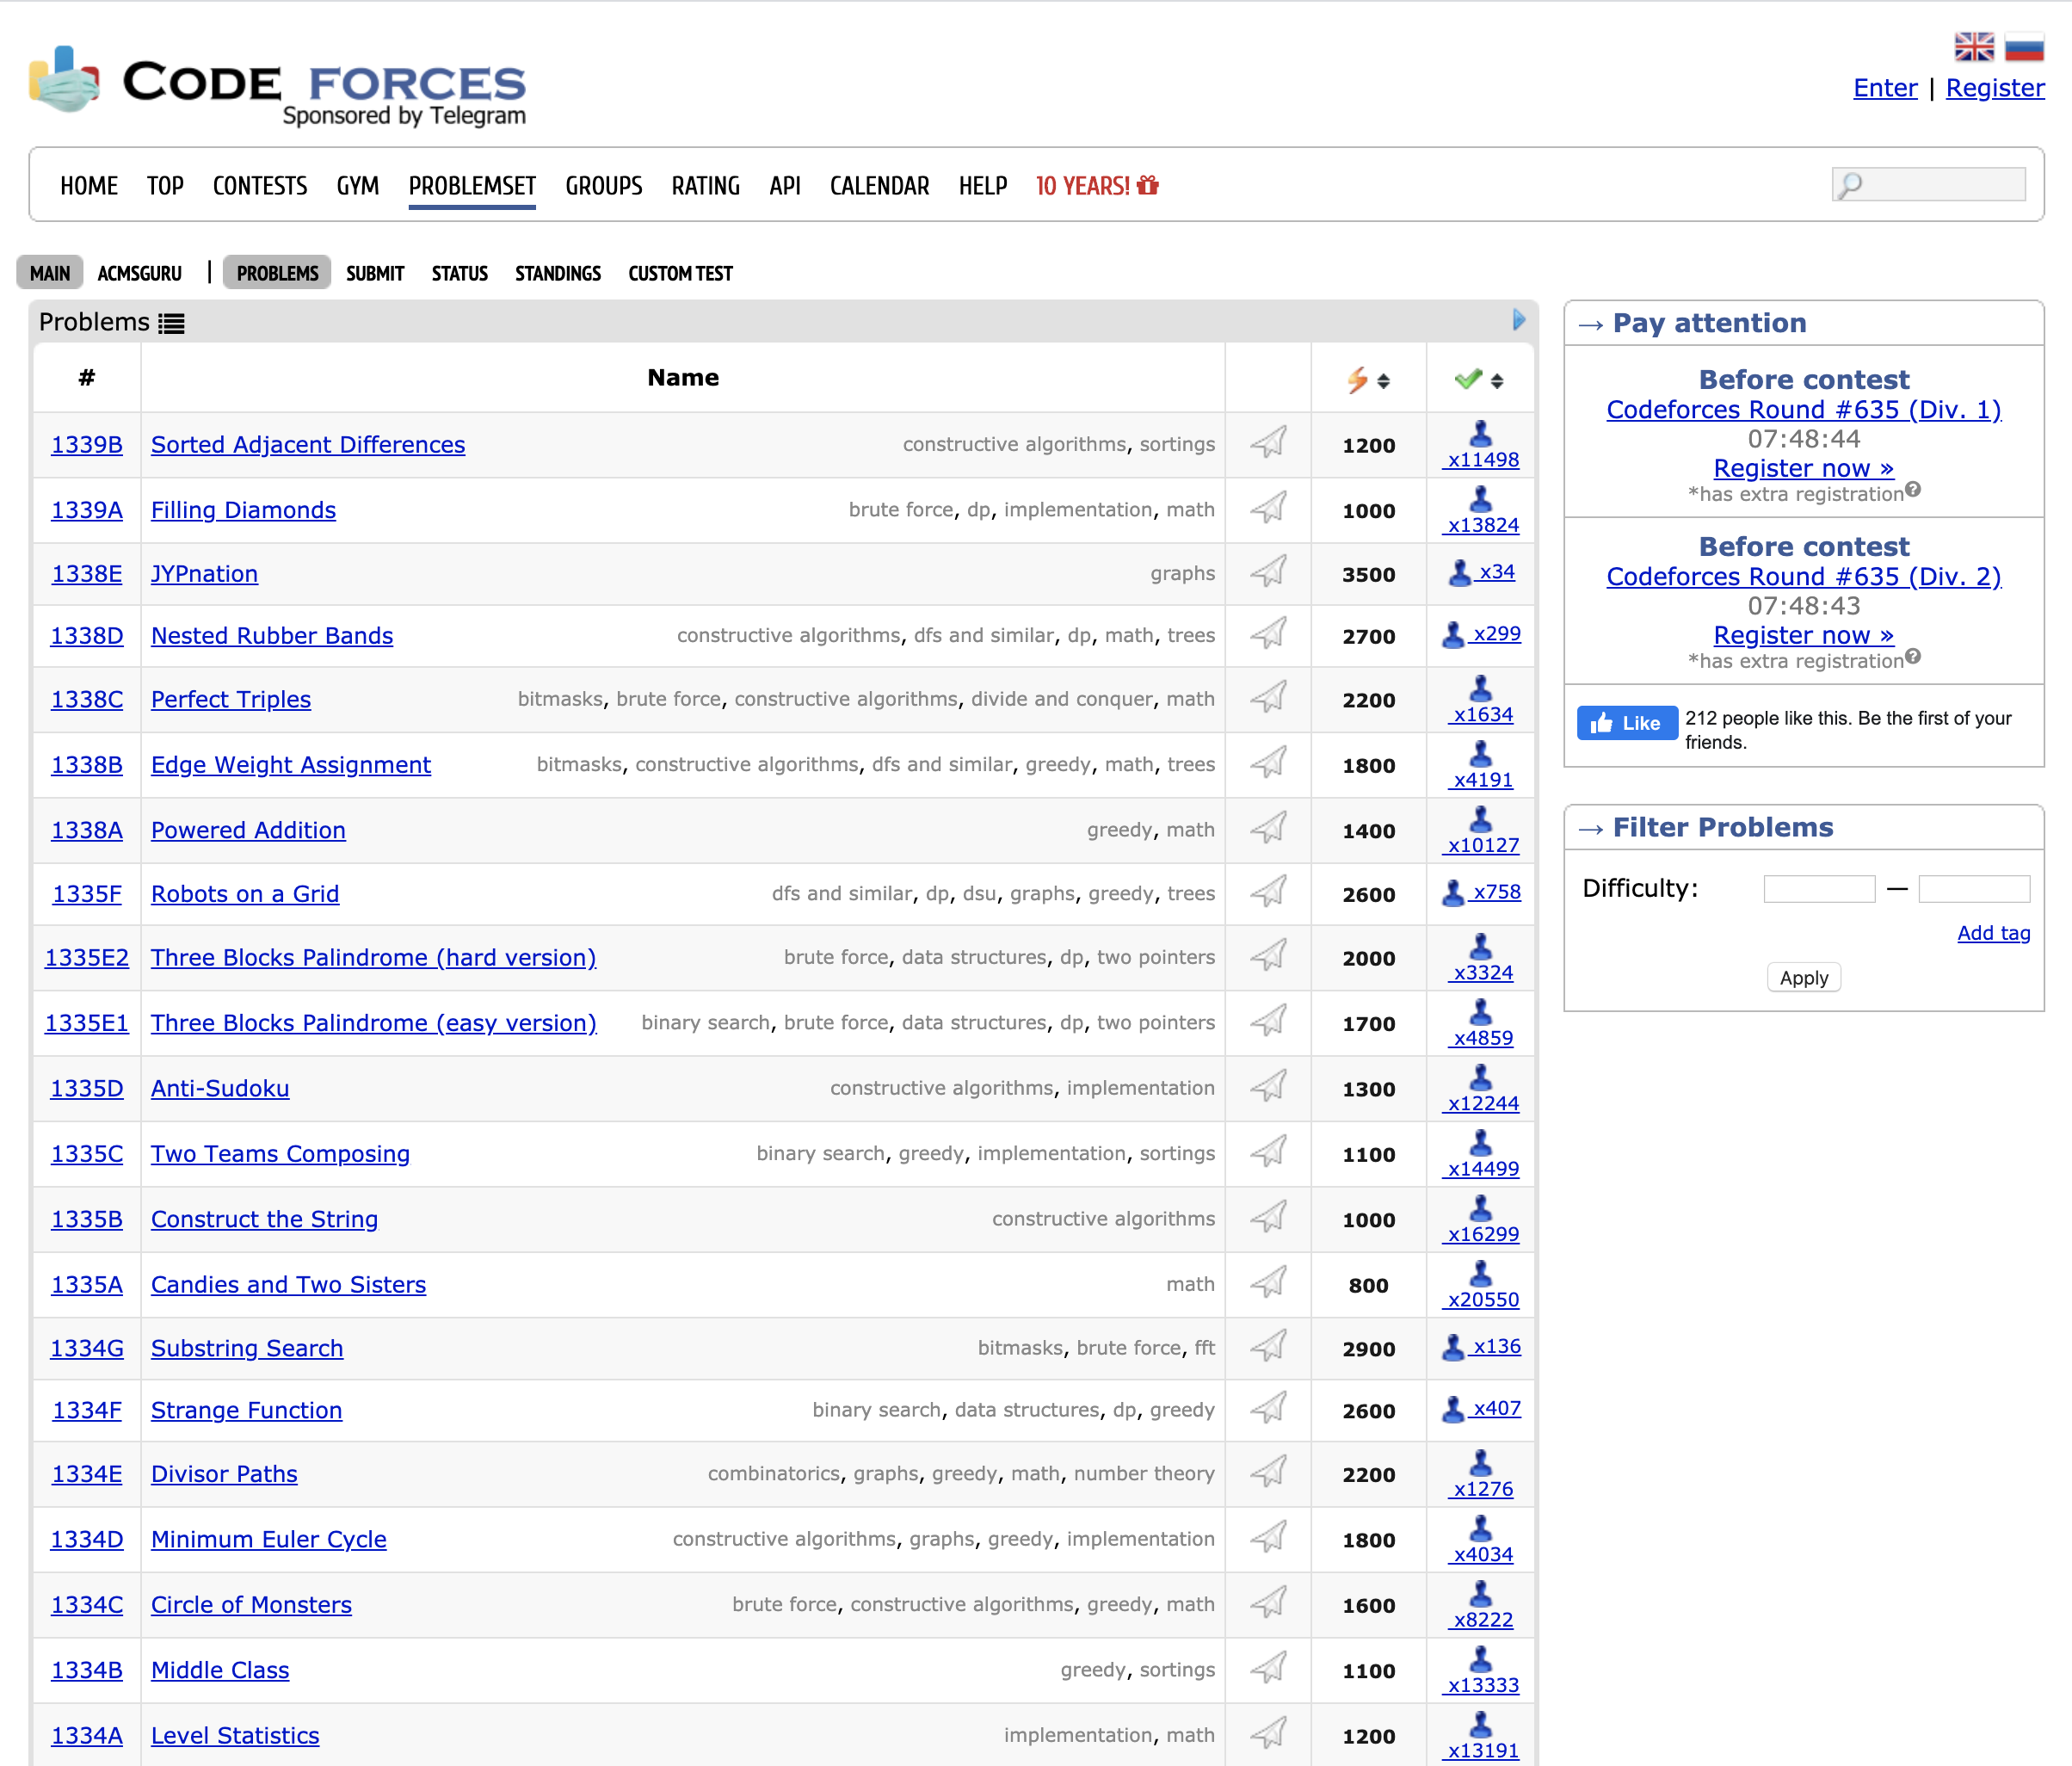
\includegraphics[width=\textwidth,height=0.6\textheight,keepaspectratio]{images/comparison/codeforces-1.png}
    \centering
    \caption[Codeforces : page de recherche de problèmes]{Page de recherche de problèmes}
\end{figure}

\begin{figure}[H]
    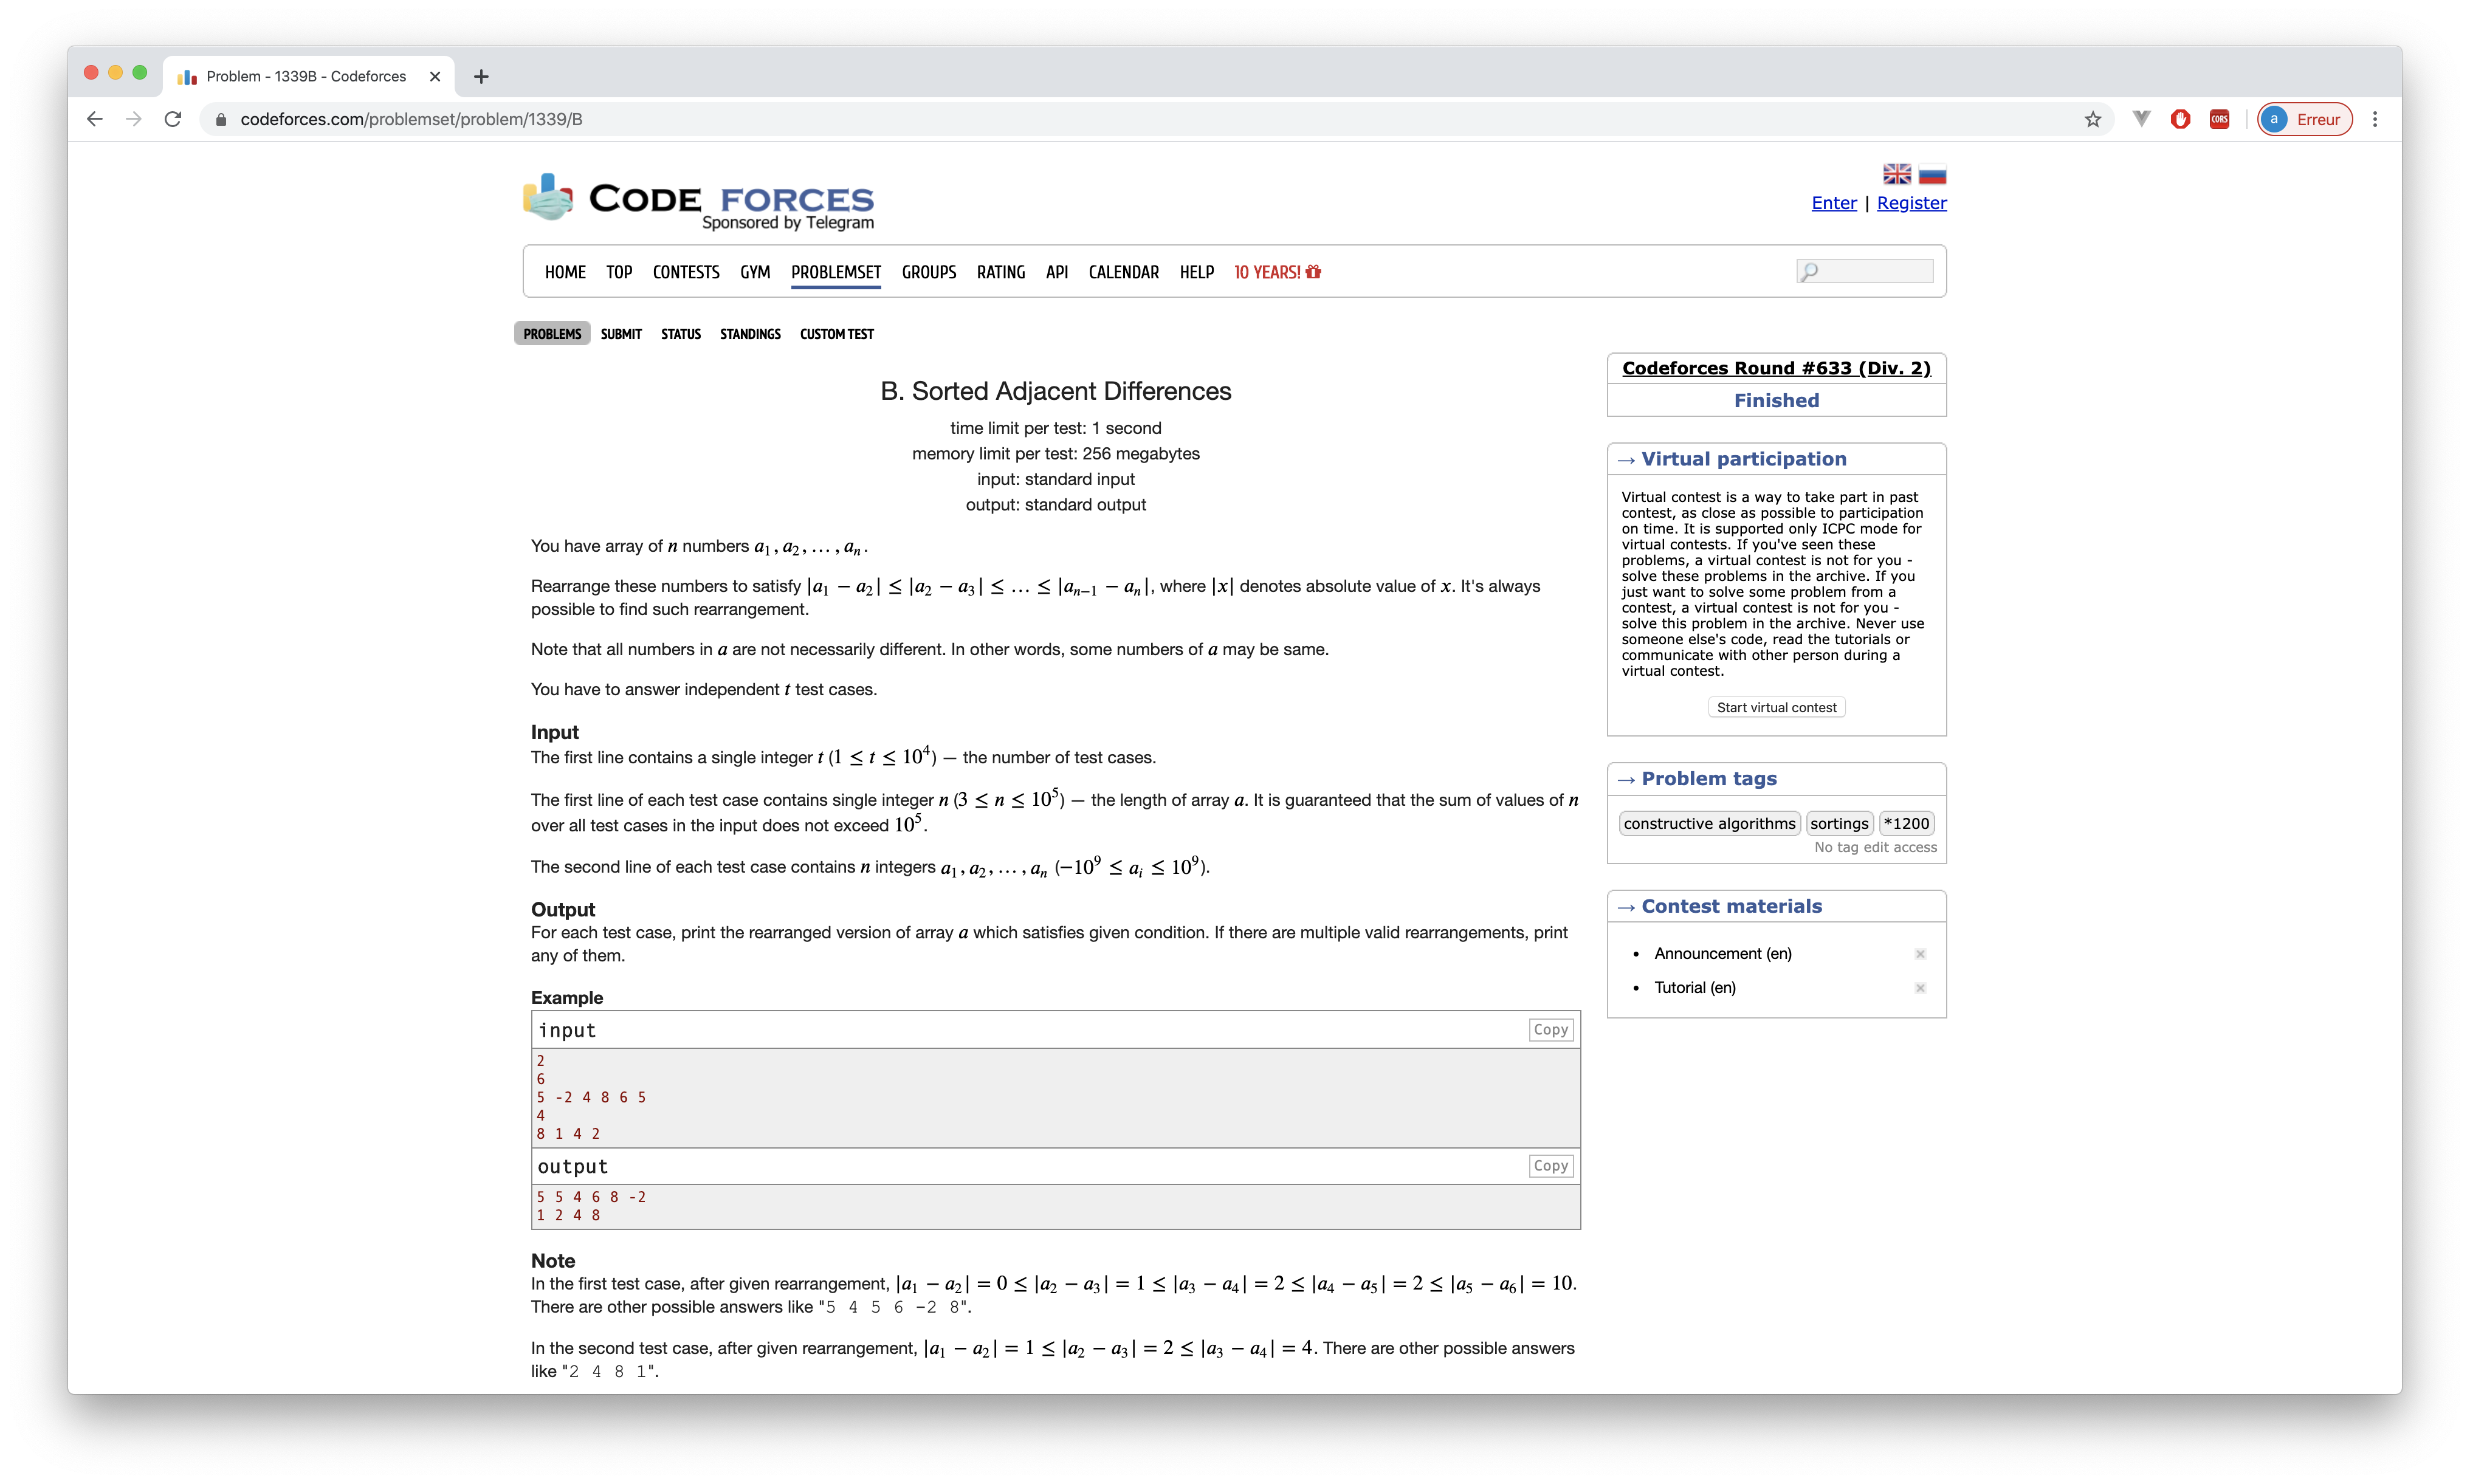
\includegraphics[width=\textwidth,height=0.6\textheight,keepaspectratio]{images/comparison/codeforces-2.png}
    \centering
    \caption[Codeforces : page d'un challenge]{Page d'un challenge}
\end{figure}


\section{Codechef}

\begin{figure}[H]
    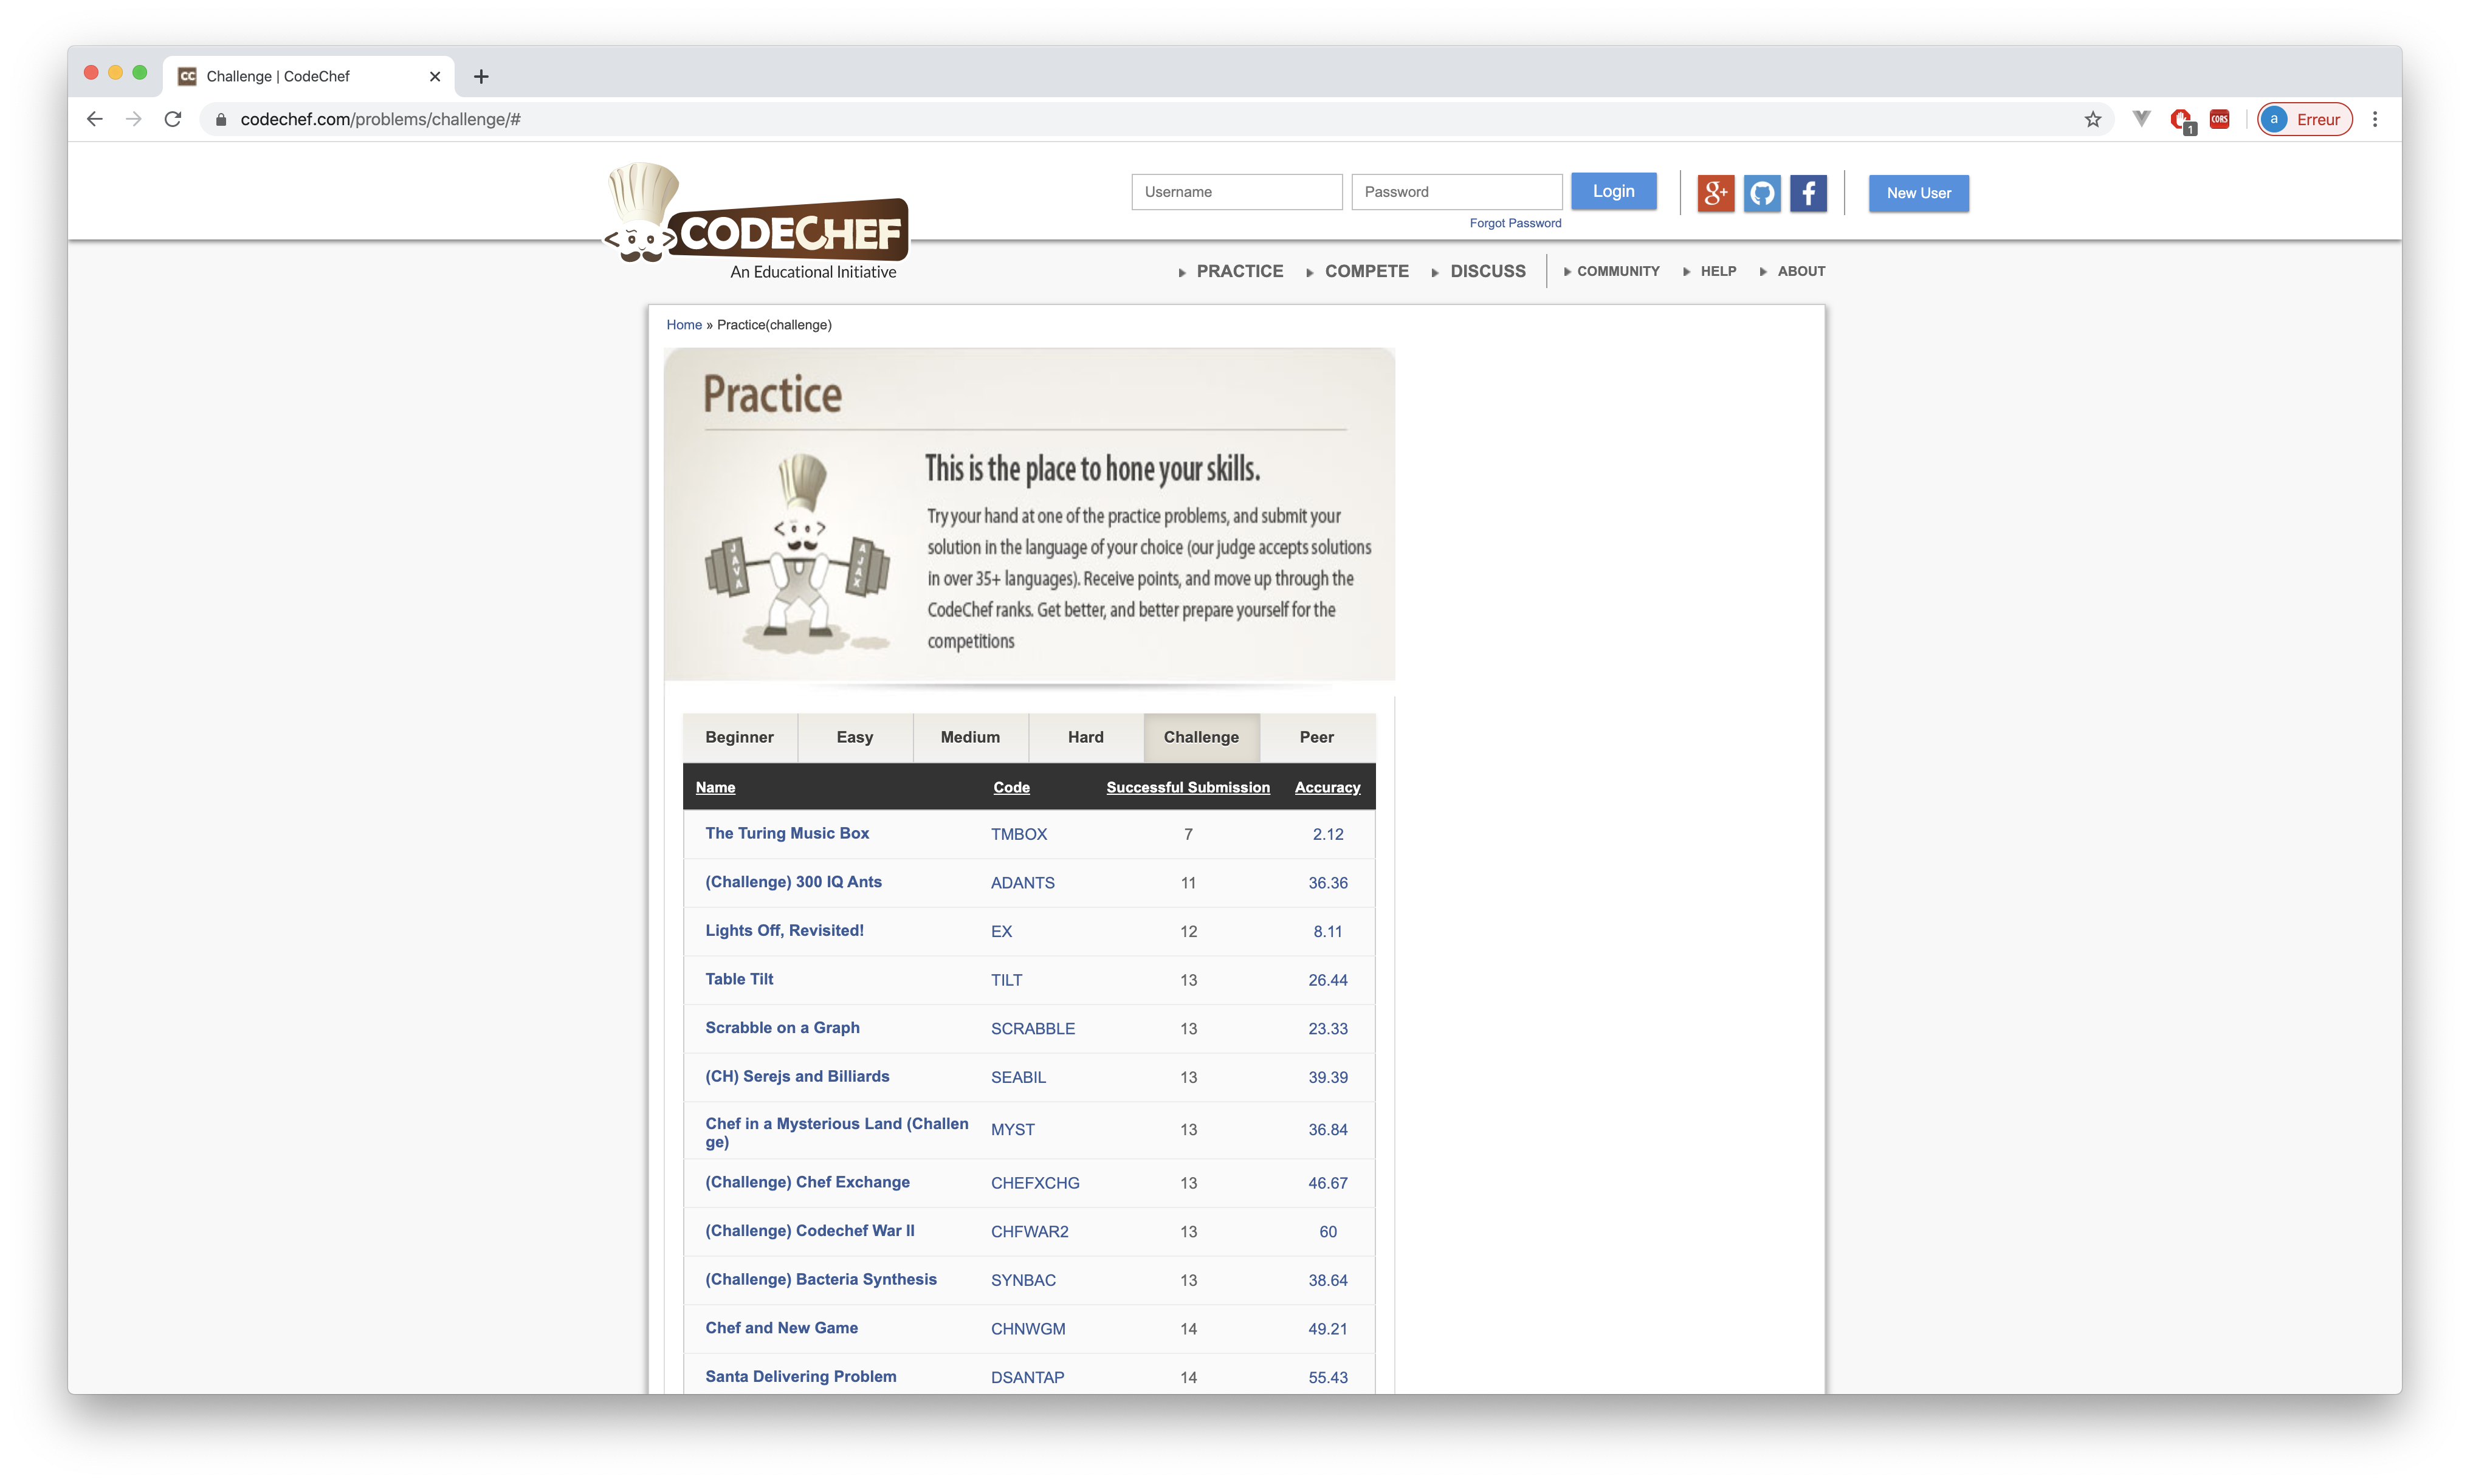
\includegraphics[width=\textwidth,height=0.6\textheight,keepaspectratio]{images/comparison/codechef-1.png}
    \centering
    \caption[Codechef : page de recherche de challenges]{Page de recherche de challenges}
\end{figure}

\begin{figure}[H]
    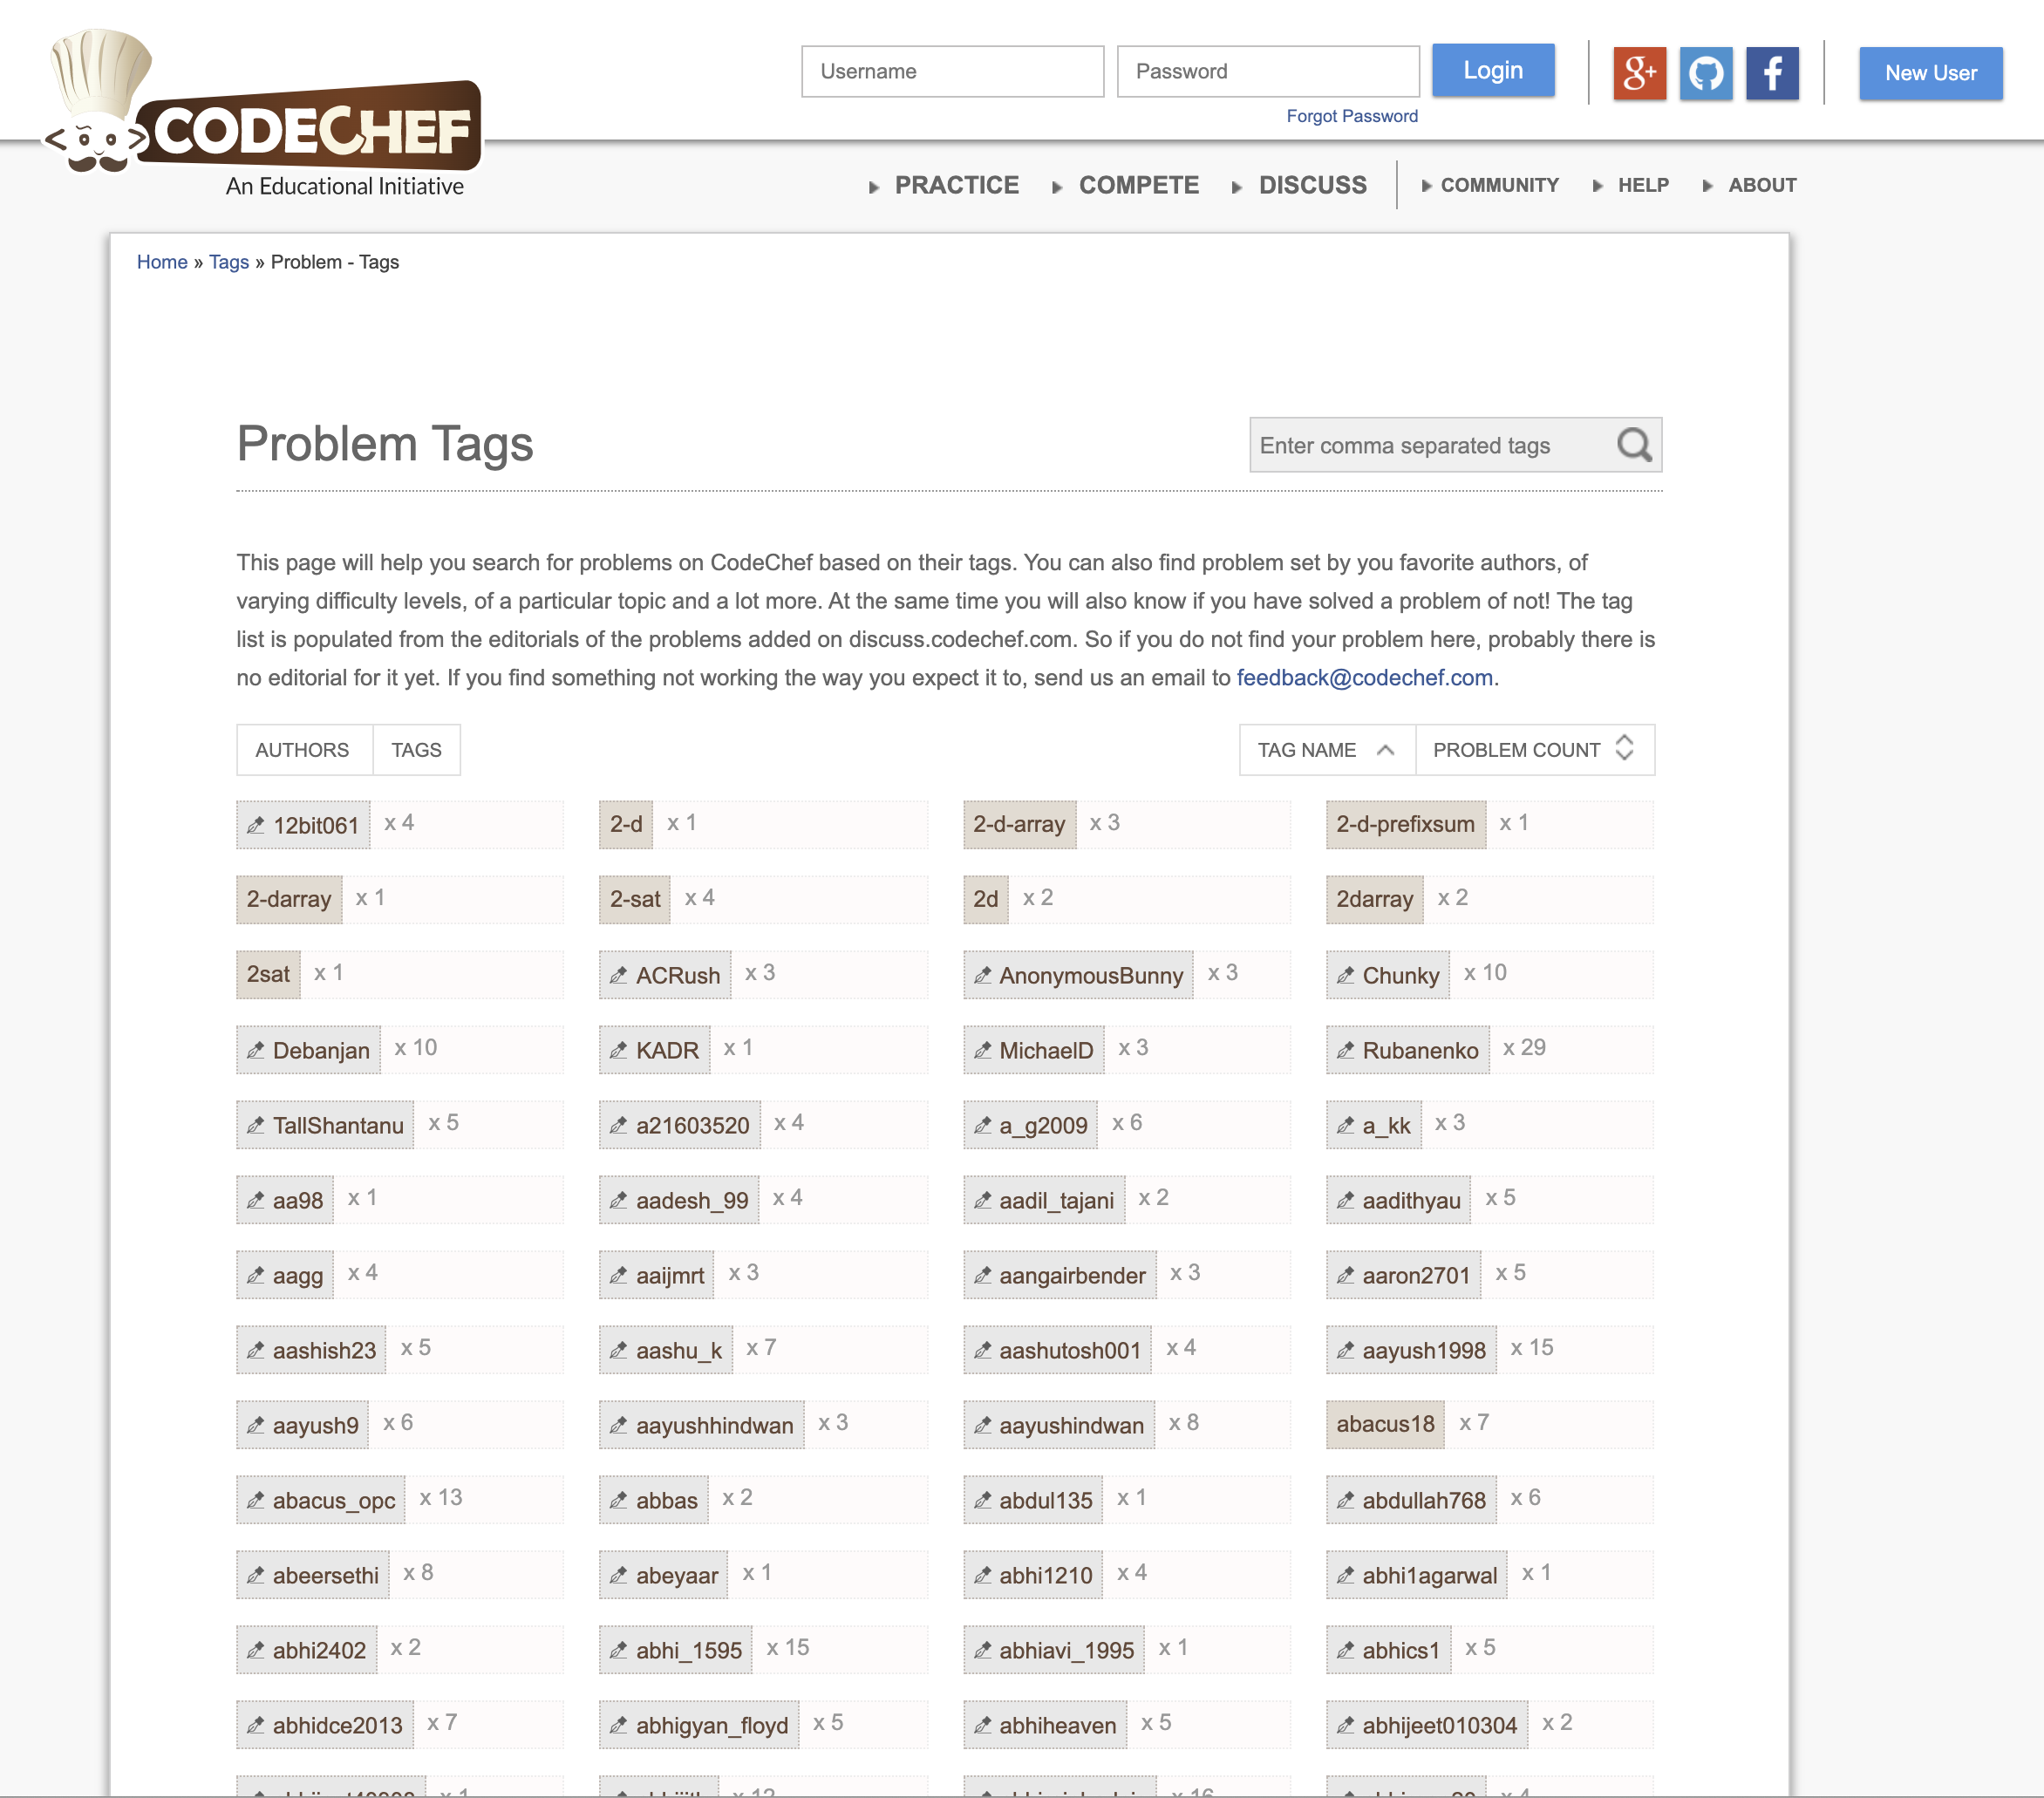
\includegraphics[width=\textwidth,height=0.45\textheight,keepaspectratio]{images/comparison/codechef-2.png}
    \centering
    \caption[Codechef : page de filtres]{Page de filtres}
\end{figure}

\begin{figure}[H]
    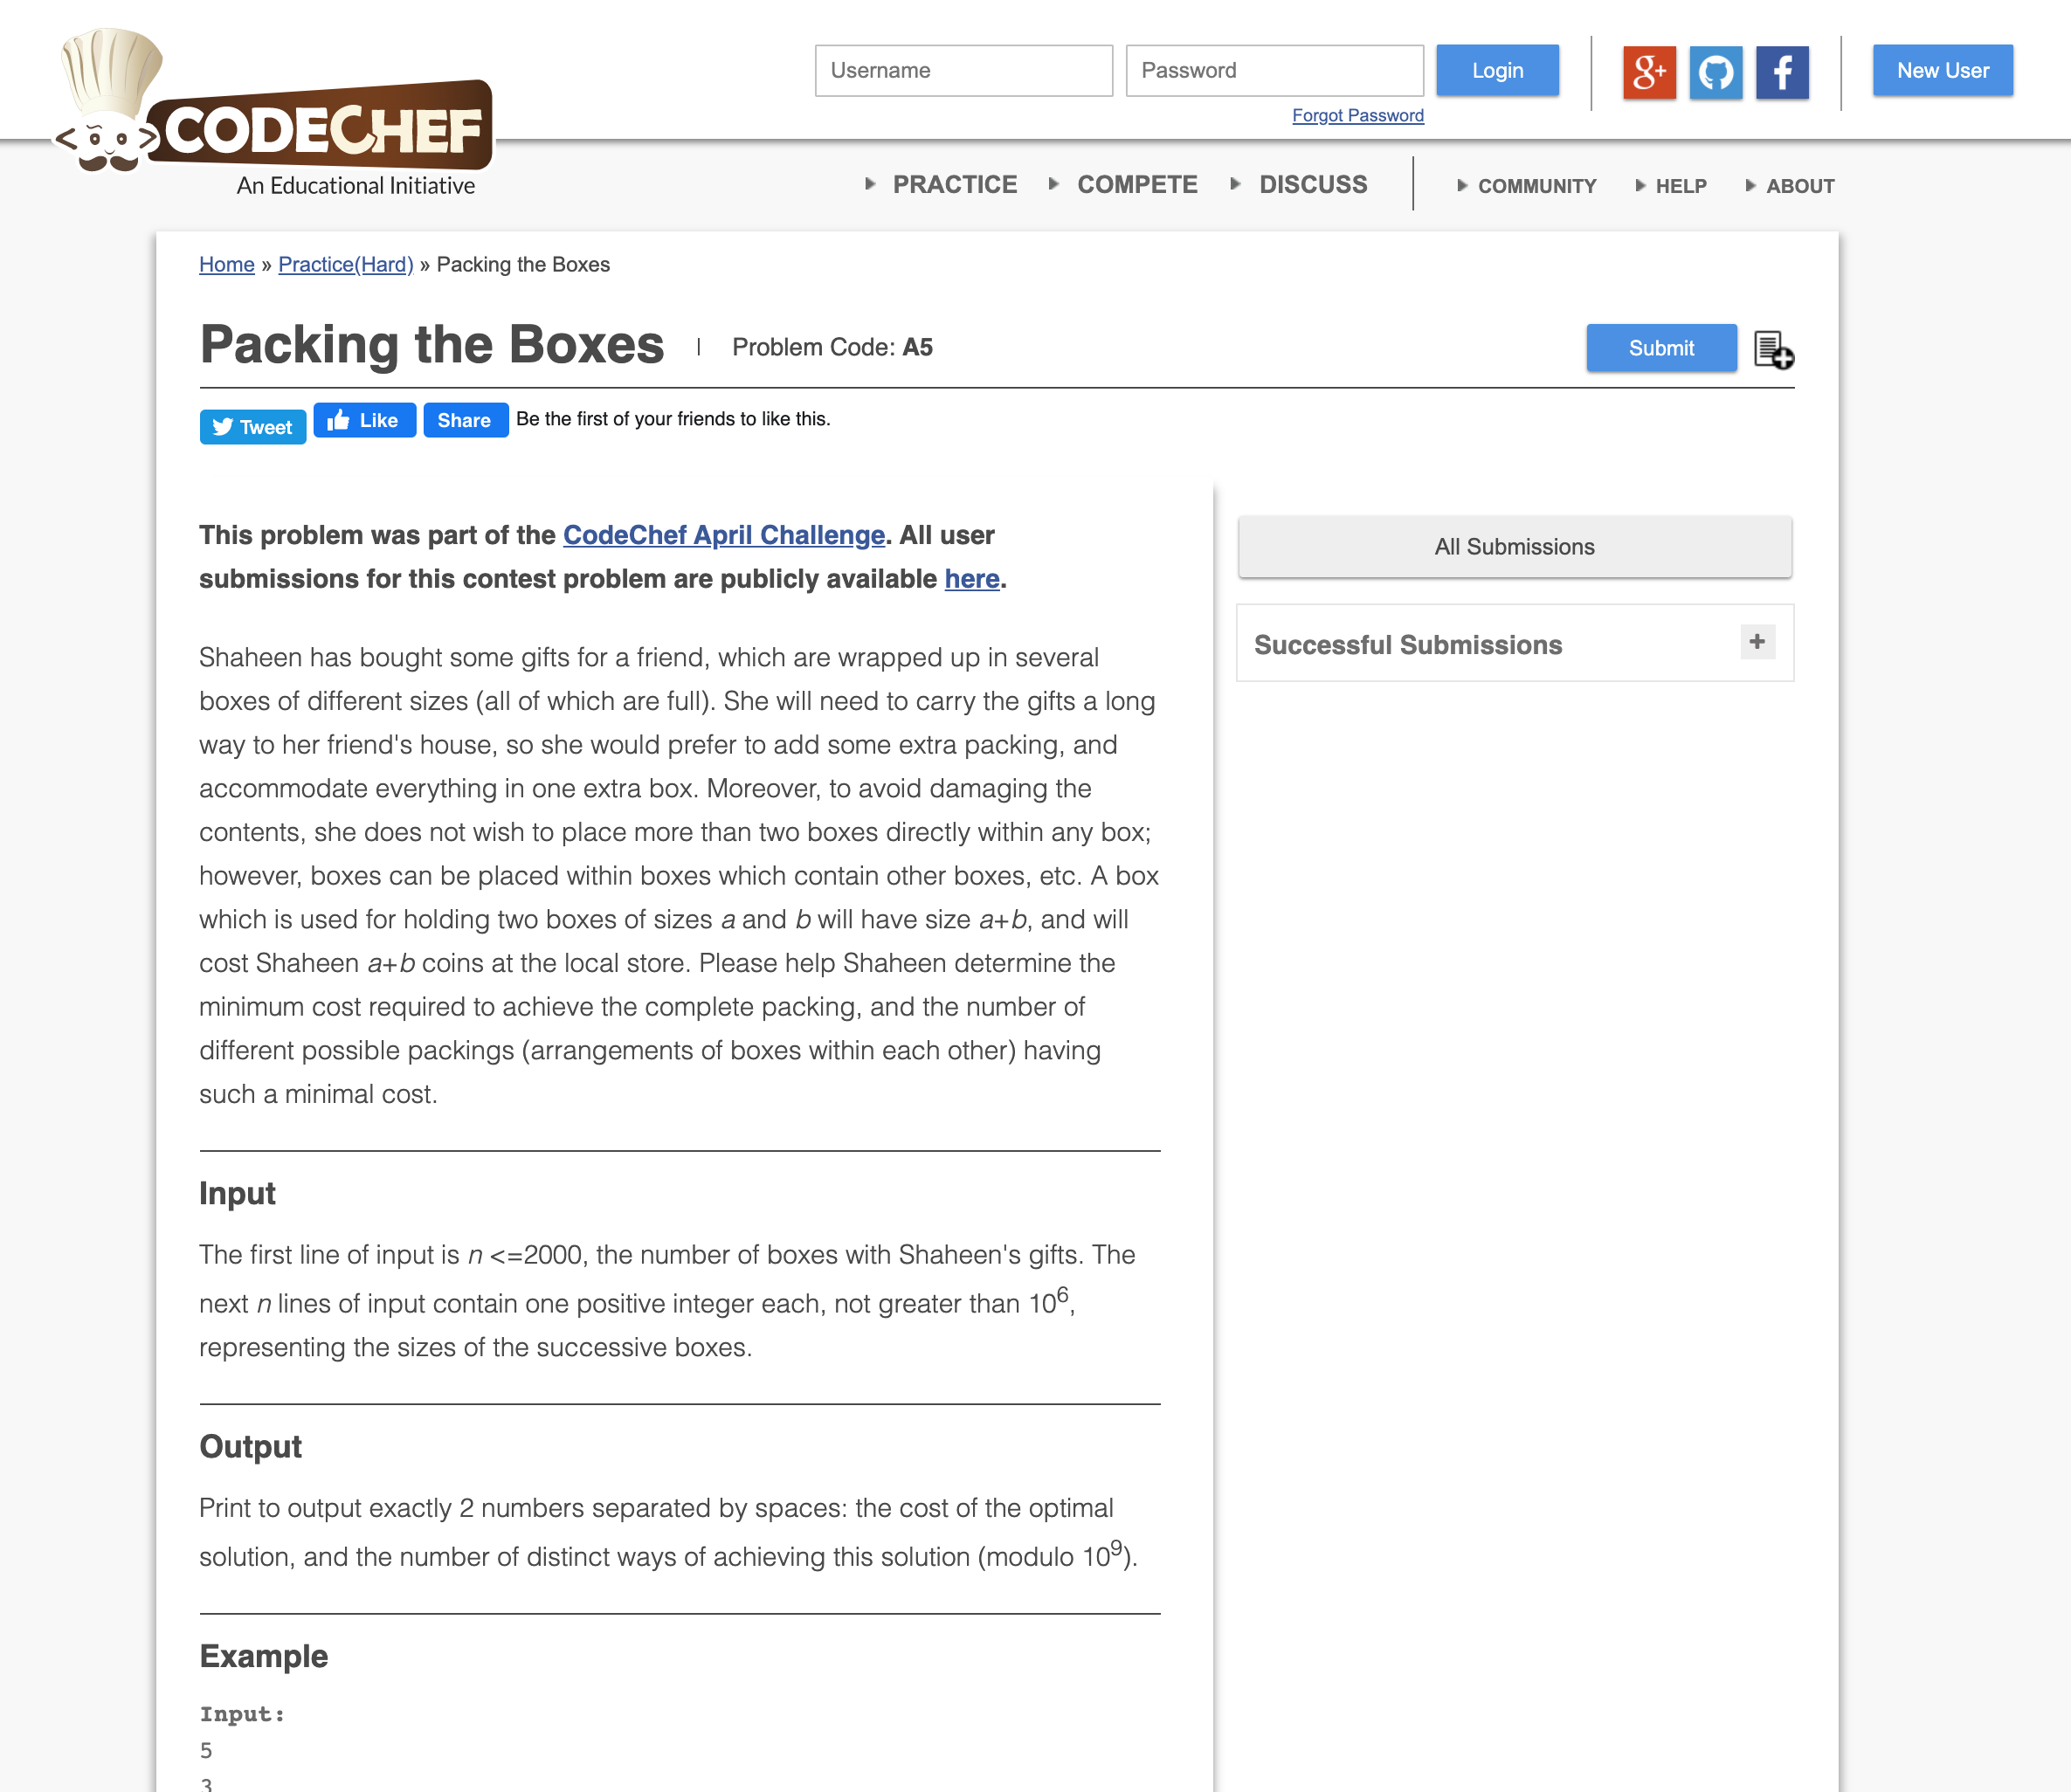
\includegraphics[width=\textwidth,height=0.45\textheight,keepaspectratio]{images/comparison/codechef-3.png}
    \centering
    \caption[Codechef : page d'un challenge]{Page d'un challenge}
\end{figure}

\section{Coderbyte}

\begin{figure}[H]
    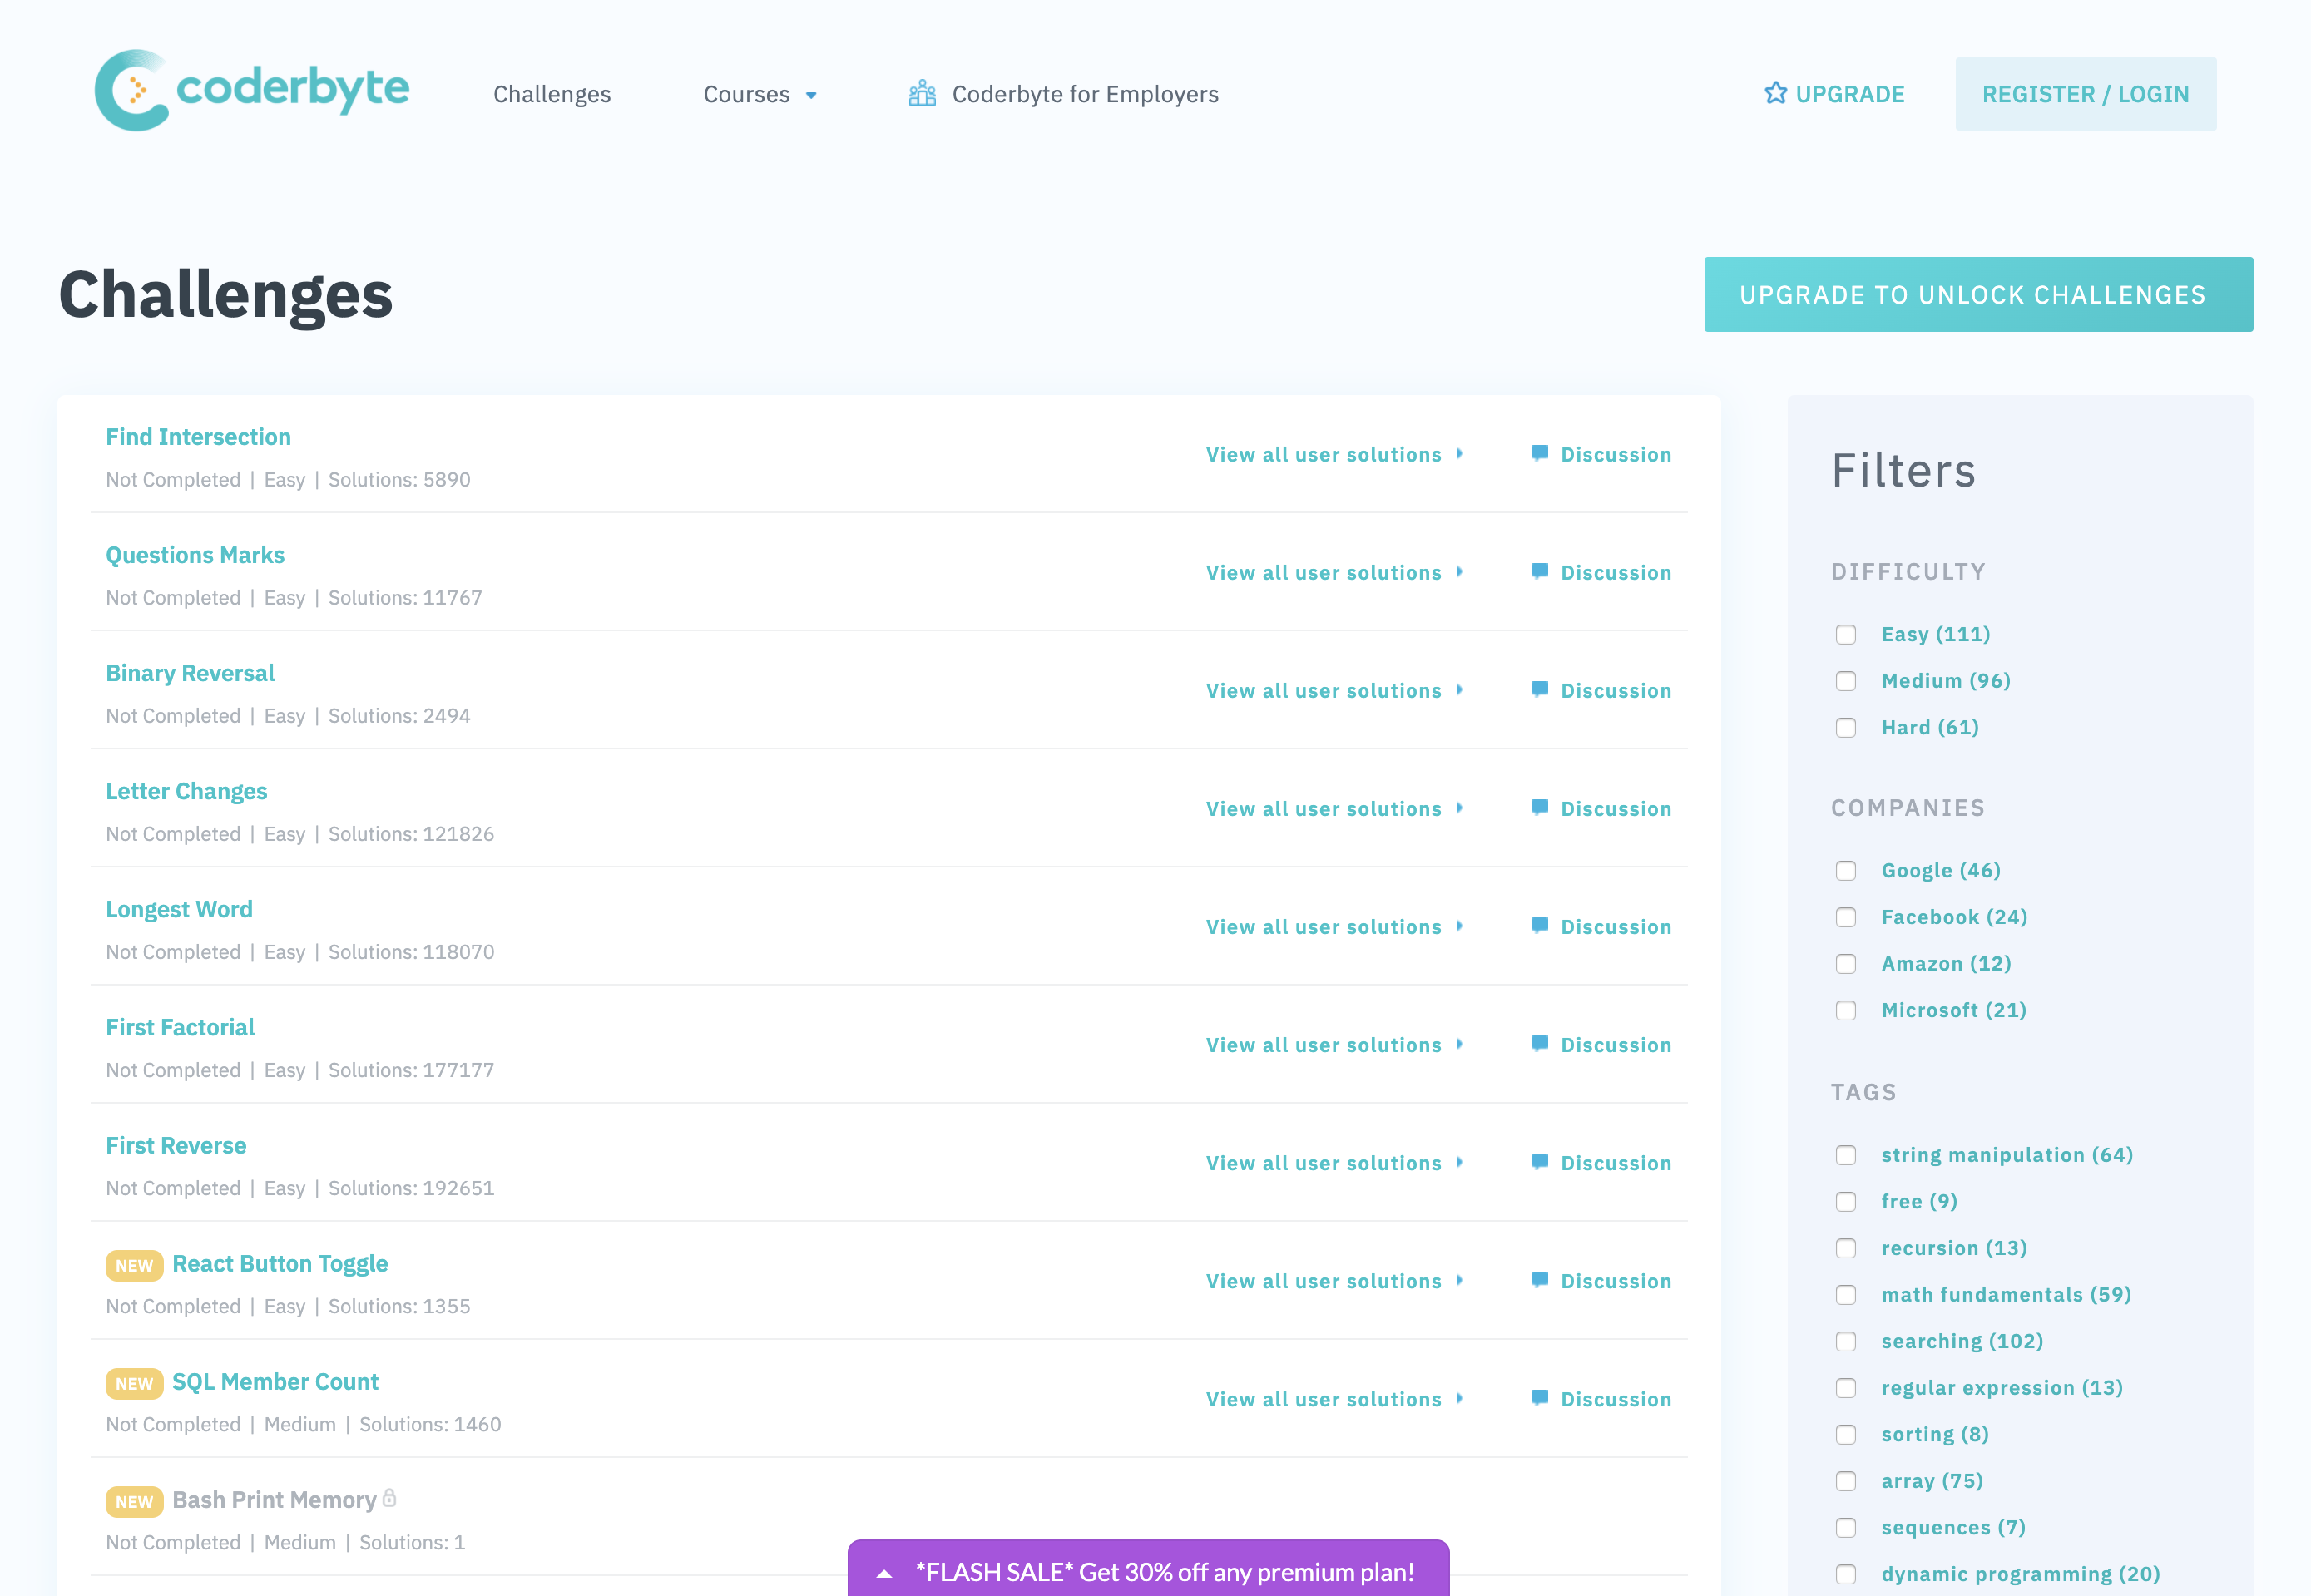
\includegraphics[width=\textwidth,height=0.5\textheight,keepaspectratio]{images/comparison/coderbyte-1.png}
    \centering
    \caption[Coderbyte : page de recherche de challenges]{Page de recherche de challenges}
\end{figure}

\begin{figure}[H]
    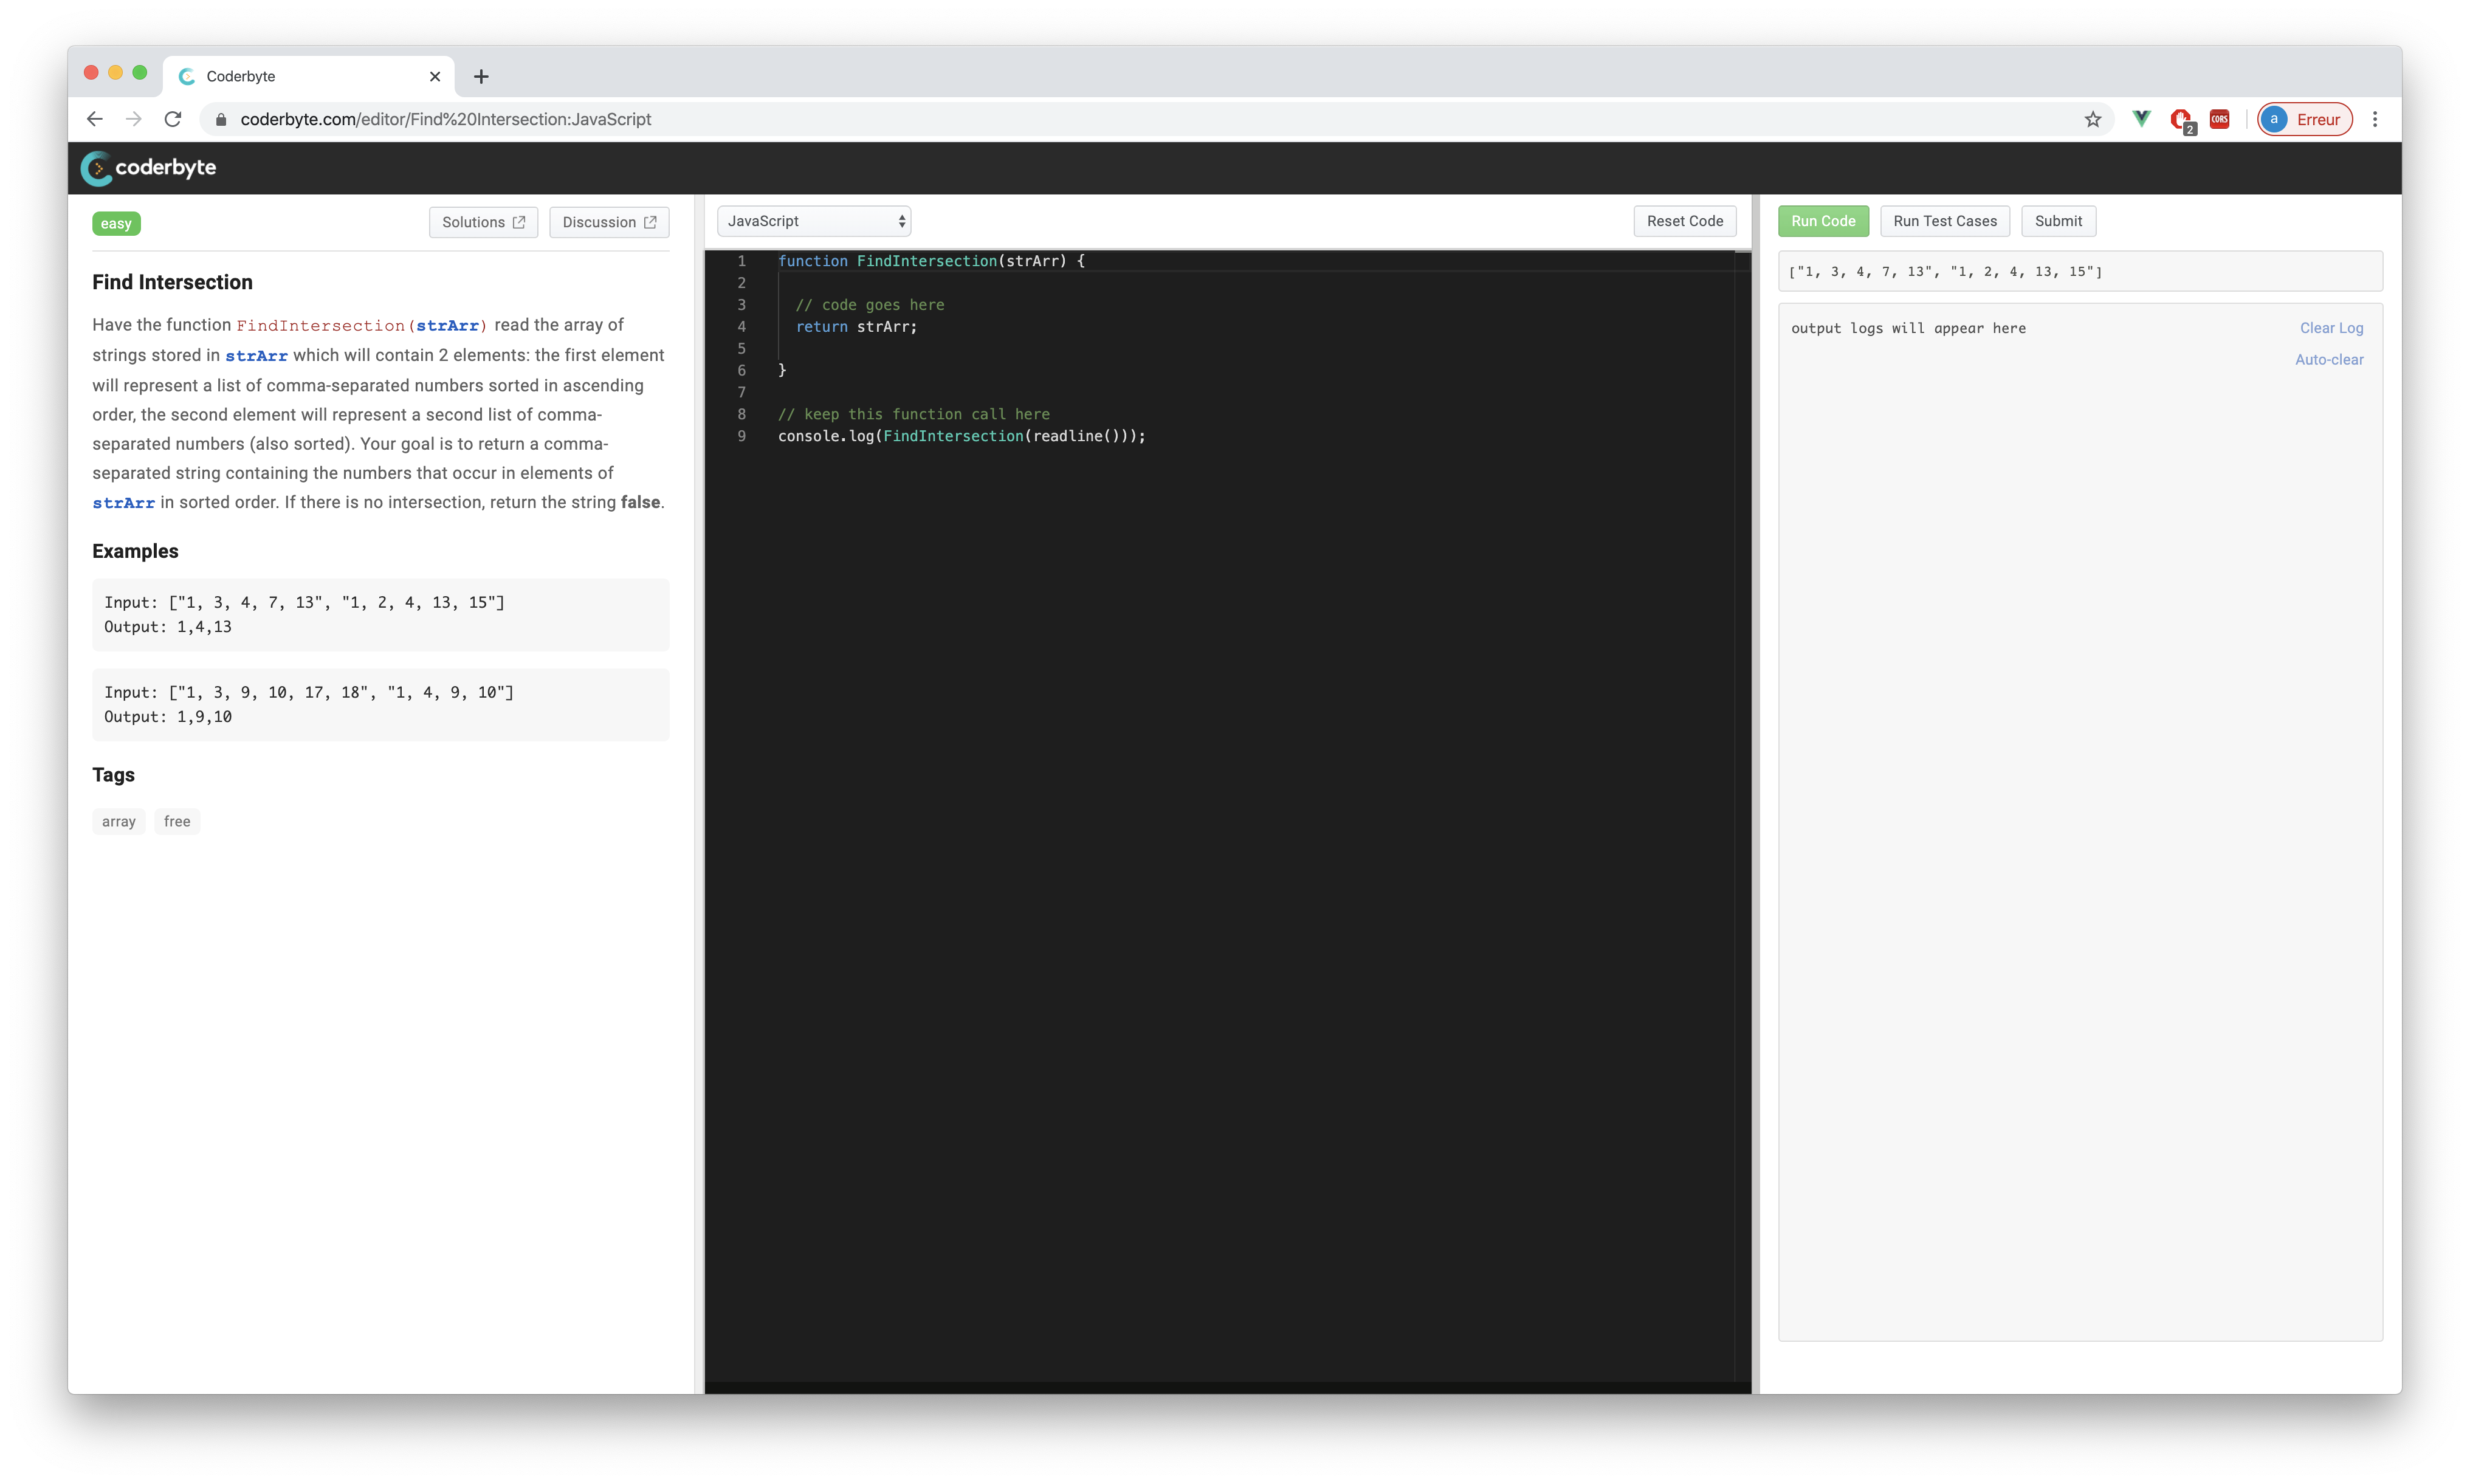
\includegraphics[width=\textwidth,height=0.35\textheight,keepaspectratio=false]{images/comparison/coderbyte-2.png}
    \centering
    \caption[Coderbyte : page d'un challenge]{Page d'un challenge}
\end{figure}


